%% 11/23/2015
%%%%%%%%%%%%%%%%%%%%%%%%%%%%%%%%%%%%%%%%%%%%%%%%%%%%%%%%%%%%%%%%%%%%%%%%%%%%
% AGUJournalTemplate.tex: this template file is for articles formatted with LaTeX
%
% This file includes commands and instructions
% given in the order necessary to produce a final output that will
% satisfy AGU requirements. 
%
% You may copy this file and give it your
% article name, and enter your text.
%
%%%%%%%%%%%%%%%%%%%%%%%%%%%%%%%%%%%%%%%%%%%%%%%%%%%%%%%%%%%%%%%%%%%%%%%%%%%%
% PLEASE DO NOT USE YOUR OWN MACROS
% DO NOT USE \newcommand, \renewcommand, or \def, etc.
%
% FOR FIGURES, DO NOT USE \psfrag or \subfigure.
% DO NOT USE \psfrag or \subfigure commands.
%%%%%%%%%%%%%%%%%%%%%%%%%%%%%%%%%%%%%%%%%%%%%%%%%%%%%%%%%%%%%%%%%%%%%%%%%%%%
%
% Step 1: Set the \documentclass
%
% There are two options for article format:
%
% 1) PLEASE USE THE DRAFT OPTION TO SUBMIT YOUR PAPERS.
% The draft option produces double spaced output.
% 
% 2) numberline will give you line numbers.

%% To submit your paper:
\documentclass[draft,linenumbers]{agujournal}
\usepackage{siunitx}
\draftfalse

%% For final version.
% \documentclass{agujournal}

% Now, type in the journal name: \journalname{<Journal Name>}

% ie, \journalname{Journal of Geophysical Research}
%% Choose from this list of Journals:
%
% JGR-Atmospheres
% JGR-Biogeosciences
% JGR-Earth Surface
% JGR-Oceans
% JGR-Planets
% JGR-Solid Earth
% JGR-Space Physics
% Global Biochemical Cycles
% Geophysical Research Letters
% Paleoceanography
% Radio Science
% Reviews of Geophysics
% Tectonics
% Space Weather
% Water Resource Research
% Geochemistry, Geophysics, Geosystems
% Journal of Advances in Modeling Earth Systems (JAMES)
% Earth's Future
% Earth and Space Science
%
%

\journalname{<enter journal name here>}


\begin{document}

%% ------------------------------------------------------------------------ %%
%  Title
% 
% (A title should be specific, informative, and brief. Use
% abbreviations only if they are defined in the abstract. Titles that
% start with general keywords then specific terms are optimized in
% searches)
%
%% ------------------------------------------------------------------------ %%

% Example: \title{This is a test title}

\title{Test}

%% ------------------------------------------------------------------------ %%
%
%  AUTHORS AND AFFILIATIONS
%
%% ------------------------------------------------------------------------ %%

% Authors are individuals who have significantly contributed to the
% research and preparation of the article. Group authors are allowed, if
% each author in the group is separately identified in an appendix.)

% List authors by first name or initial followed by last name and
% separated by commas. Use \affil{} to number affiliations, and
% \thanks{} for author notes.  
% Additional author notes should be indicated with \thanks{} (for
% example, for current addresses). 

% Example: \authors{A. B. Author\affil{1}\thanks{Current address, Antartica}, B. C. Author\affil{2,3}, and D. E.
% Author\affil{3,4}\thanks{Also funded by Monsanto.}}

\authors{Alexander Beck\affil{1}, Jan Henneberger\affil{1}, and Ulrike Lohmann\affil{1}}


% \affiliation{1}{First Affiliation}
% \affiliation{2}{Second Affiliation}
% \affiliation{3}{Third Affiliation}
% \affiliation{4}{Fourth Affiliation}

\affiliation{1}{Institute for Atmospheric and Climate Sciences, ETH Zurich, Zurich, Switzerland}
%(repeat as many times as is necessary)

%% Corresponding Author:
% Corresponding author mailing address and e-mail address:

% (include name and email addresses of the corresponding author.  More
% than one corresponding author is allowed in this LaTeX file and for
% publication; but only one corresponding author is allowed in our
% editorial system.)  

% Example: \correspondingauthor{First and Last Name}{email@address.edu}

\correspondingauthor{Jan Henneberger}{janhenneberger@env.ethz.ch}

%% Keypoints, final entry on title page.

% Example: 
% \begin{keypoints}
% \item	List up to three key points (at least one is required)
% \item	Key Points summarize the main points and conclusions of the article
% \item	Each must be 100 characters or less with no special characters or punctuation 
% \end{keypoints}

%  List up to three key points (at least one is required)
%  Key Points summarize the main points and conclusions of the article
%  Each must be 100 characters or less with no special characters or punctuation 

\begin{keypoints}
\item  In-situ measurements of microphysical cloud properties with a holographic Imager
\item  Influence of in-situ cloud observations at mountain top stations by ground based ice enhancement processes 
\item
\end{keypoints}

%% ------------------------------------------------------------------------ %%
%
%  ABSTRACT
%
% A good abstract will begin with a short description of the problem
% being addressed, briefly describe the new data or analyses, then
% briefly states the main conclusion(s) and how they are supported and
% uncertainties. 
%% ------------------------------------------------------------------------ %%

%% \begin{abstract} starts the second page 

\begin{abstract}
In-situ cloud observations at mountain top research station regularly measure an ice crystal number concentration orders of magnitudes higher than expected from measurements or simulations of ice nuclei. The source of the majority of the observed ice crystals still remains an enigma. Several studies suggest a strong influence of mountain top in-situ measurements by surface based ice enhancement process, e.g. blowing snow, hoar frost or riming on trees, rocks and the snow surface. In this case the relevance of in-situ observations on mountain top stations end/or a possible impact of such a surface based ice enhancement process on orographic clouds has to be further investigated.

In this study we assess the influence of surface based ice enhancement processes on in-situ cloud observations at mountain top stations. Therefore, vertical profiles within a height of 10\,\si{m} above the snow covered surface were observed at the Sonnblick Observatory in the Hohen Tauern Region, Austria. Results show that the ice crystal number concentration  decreases by at least factor of 2 within a height interval of 7.5\,\si{m} if the Sonnblick Observatory was in cloud. During a short time period when the Sonnblick Observatory was not in cloud an ice crystal number concentration of several hundreds per liter was observed at a height of 2.5\,\si{m} an decreased to 10 per liter within a height interval of 7.5\,\si{m} at a wind speed of 10\,\si{m\,s^{-1}}. These observations strongly suggest that mountain top in-situ measruements are highly influenced by surface based ice enhancement processes. 
\end{abstract}


\section{Introduction}
The microphysical properties of orographic clouds, e.g. their phase composition an cloud processes are key parameters for the clouds lifetime, extent, as well as the intensity of precipitation they produce \citep{Rot07}. On the other hand these parameters influence the radiative properties of midlevel clouds in the temperature range between 0 to -35\,\si{^\circ C}. Compared to a purely liquid cloud in this temperature range an ice cloud reflects 17\,\si{W\,m^{-2}} more radiation than an pure ice cloud \citep{Loh02}. A well representation of orographic clouds is therefore crucial for accurate weather predictions in alpine terrain and improved climate models. 

Because our understanding of fundamental processes of especially orographic mixed-phase clouds is still limited \citep{Bau10}, in-situ measurements are important and frequently conducted at mountain top research stations. Despite an improved understanding on the origin of ice crystals from nucleation (citation!!!!) as well as from secondary ice multiplication processes \citep{Fie17} the source of most of the ice crystals observed at mountain top stations remains an enigma (citation!!!!). 

A study at the Elk Mountain reports ice crystal number concentrations on the order of several hundreds per liter close to the surface which was three orders of magnitude higher than observed on an aircraft aloft \citep{Rog87}. Secondary ice multiplication processes like fragmentation \citep{Ran01} or the Hallett-Mossop process \citep{Hal74} were ruled out by the authors due to the lack of large ice crystals, respectively large cloud droplets. Instead they proposed blowing snow as a surface based ice crystal source to generate such enormous ice crystal number concentrations near the snow surface. Ice crystal number concentrations in the order of 1000 per liter were also observed near the surface on the Antarctica Peninsula \citep{Lac01}. They used formvar replica collected at a height of 2\,\si{m} above the surface measure ice crystal number concentrations and suggested that the ice crystals originate from the snow covered surface. \citet{Loy15} reported ice crystal number concentrations of up to 2000 per liter during the INUPIAQ project in February 2014 at the Jungfraujoch, Switzerland. They also ruled out secondary ice multiplication mechanisms as a possible source of these enormous ice crystal number concentrations. However, they also ruled out blowing snow as the source for ice crystal number concentrations larger than 100 per liter, because no correlation of the ice crystal number concentration with wind speed was observed. Instead, they suggested hoar frost as a wind independent, surface based ice multiplication process to cause such high ice crystal number concentrations. Although these studies use different mechanisms to explain their measured ice crystal number concentration, they agree on an strong influence by surface based processes. 

While the influence of mountain top measurements by surface based processes is widely accepted, the impact of the resuspended ice crystals on the development of a supercooled oropgraphic cloud, e.g. a more rapid glaciation and enhanced precipitation has not been studied extensively \citep{Gee15}. 

The properties of blowing snow have been studied in the context of snow redistribution ("snow drift") and reduced visibility due to the resuspended ice crystals. Usually the properties of the ice crystals were observed up to several meters above the snow surface \citet{Sch82, Nis05}. It has been reported that blowing snow occurs above a wind speed threshold that varies between 4\,\si{m\,s^{-1}} and 13\,\si{m\,s^{-1}} \citep{Bro88, Li97, Mah03, Der99}. Other than wind speed the concentration of blowing snow is controlled by snowpack properties (type of snow that fell, temperature and humidity of the snow pack, solar radiation and tree shadows) and atmospheric conditions (temperature, ) \citep{Vio13}. \citet{Sch82} observed that the ice crystal concentration decreases within one meter above the surface with the power of -0.5 to -1.1. \citet{Nis05} extended these measurements to a height of 9.6\,\si{m}. They found that the ice crystal concentration usually decreases to as low as 1-10 particles per liter at a height of 9.6\,\si{m} and the relative importance of the small ice crystals below < 100\,\si{\mu m} during a precipitation event decreases from nearly 100\,\si{\%} at 1.1\,\si{m} to below 20\,\si{\%} at 9.6\,\si{m}. With a rapid decrease in the ice crystals number concentration observed by these studies the impact of blowing snow on orographic clouds may be limited. However, most of these studies were conducted in dry air conditions where ice crystals undergo rapid sublimation \citep{Yan08}, which may limit the applicability of these results. For hoar frost only one modeling study exists to our knowledge. \citet{Far15} implemented a flux of surface hoar crystals in the WRF model based on a frost flower aerosol flux to simulate ice crystal concentrations measured at the Jungfraujoch by \citet{Llo15}. They also found, that the surface ice crystals are not advected high into the atmosphere, limiting their impact on orographic clouds. They also suggest that more measurements on the ice crystal flux from the snow covered surface are necessary to simulate the impact of surface based ice crystal enhancement processes on the development of orographic clouds.

In contrast to these finding are several remote sensing studies exist, which suggest an influence by ice crystals advected from the surface as high as 1\,\si{km} into the atmosphere. Satellite observations of Blowing Snow from MODIS and CALIOP exist over the Antarctica \citep{Pal01}. They observed layer thicknesses up to 1\,\si{km} with an average thickness of 120\,\si{m} for all observed blowing snow events. Similar observations from lidar measurements exist from the South Pole with an observed layer thickness of ice crystals of usually less than 400\,\si{m} \citep{Mah03} and some rare cases when a subvisual layer exceeded a height of 1\,\si{km}. However, a possible suspension of clear-sky precipitation could not be ruled out as a source of the observed ice crystal layers. Observations of layers of ice crystals also exist from radar measurements on an aircraft in the vicinity of the Medicine Bow Mountains \citep{Val12}. The observed ground-layer snow clouds were most of the time not visually detectable but produced a radar signal. Possible origin of ice crystals producing such ground-layer snow clouds are resuspended ice crystals from the surface or riming of cloud droplets at the surface. \citet{Gee15} presented evidence for ice crystals becoming lofted up to 250\,\si{m} in the atmosphere by boundary layer separation behind terrain crests and by hydraulic jumps. They also found evidence that ice crystals from the surface may lead to the glaciation of supercooled orographic clouds and enhanced precipitation. However, \citet{Gee15} also mention the limitation of radar and lidar measurement to seperate the small ice crystals produced by surface processes from the larger falling snow particles and more aboundant cloud droplets. They even suggest "to explore BIP lofting into orographic clouds, ice particle imaging devices need to be installed on a tall tower, or on a very steep mountain like the Jungfraujoch".

In this study we assess the impact of surface based ice enhancement process, e.g blowing snow or hoar frost on in-situ cloud observations at mountain top stations and a possible influence of orographic mixed-phase clouds. Therefore, for the first time, vertical profiles of surface based ice crystal production within a height of 10\,\si{m} above the surface were observed in cloud at the Sonnblick Observatory. 

This paper is structured as follows. The measurement site and set up of the field campaign are described in Section \ref{}. The results are presented in section \ref{Results}. In section \ref{Discussion} the results are discussed and put in the context of earlier findings. A short summary is presented in section \ref{summary}. 

\section{Field Measurements at the Sonnblick Observatory}
\label{sectionMeasurementSite}

\subsection{Site description}

This field campaign was conducted at the Sonnblick Observatory (SBO) situated at the summit of Mt. Sonnblick at 3106\,\si{masl} (\ang{12;57;}E, \ang{47;03;}N) in the Hohen Tauern National Park in the Austrian Alps. The SBO is a meteorological observatory operated all year by the ZAMG (Central Institute for Meteorology and Geodynamics). On the East and South the SBO is surrounded by large glacier fields with a moderate slope, whereas on the Northeast a steep wall of approximately 800\,\si{m} descends to the valley (Fig.~\ref{fig:SetUp}, right). Part of the SBO is a 15\,\si{m} high tower used for meteorological measurements by the ZAMG. The data presented in this paper was collected during a field campaign in February 2017. 

\subsection{Instrumentation}
The microphysical properties of clouds, hydrometeors and resuspended particles from the surface were observed with the HoloGondel platform \citep{bec17}. For this, the HoloGondel platform was mounted on an elevator that was attached to the meteorological tower of the SBO (Fig.~\ref{fig:Elevator}) to obtain vertical profiles of the microphysical properties within a height interval of 12\,\si{m} above the surface where the platform was repeatedly positioned at five different heights as indicated in Figure \ref{fig:Elevator}. On the Elevator the HoloGondel platform had a distance of approximately 1.5\,\si{m} from the tower and was oriented in a way that the sampled air with the holographic imager HOLIMO 3G, which is the main part of the HoloGondel platform, was undisturbed during North and South wind cases. HOLIMO 3G captures the information of a three-dimensional volume of air containing cloud particles on a single image with a sample area of 20\,\si{mm} x 13.4\,\si{mm}. In this study the examined volume has a depth of 60\,\si{mm} along the optical axis resulting in a sample volume of 16\,\si{cm^3}. The open source software HoloSuite \citep{Fug15} is used to reconstruct the in-focus images of the particles. Particles smaller than 25\,\si{\um m} are classified as liquid droplets, whereas particles larger than 25\,\si{\um m} are separated in liquid droplets and ice crystals based on the shape of their 2D image. Similar to a study by \cite{Sch17} the ice crystals were further visually classified into three different groups: regular, irregular and aggregates. Because the visual classification of several thousands of ice crystals is time consuming. this subclassificaition of ice crystals was done only for the profiles on February 17th.

%The CIP was located on the north facing side of the measurement terrace of the SBO (see Fig.~\ref{fig:SetUp}, left). Because this location is in the wind shadow of the building of the SBO during south wind cases, the CIP data is only analysed for February 17th, when the wind direction was from North.  
Meteorological data are available from the measurements by the ZAMG and the HoloGondel platform. The ZAMG measures one minute averages of temperature, relative humidity and horizontal wind speed and direction at the top of the meteorological tower. Snow cover depth is daily manually observed by the operators of the SBO. Based on these measurements the change of the snow cover is calculated. However, this calculation includes all the changes in the snow cover depth, e.g. snow drift, sublimation, melting and fresh snow. Daily measurements of the total precipitation are available on the North and South side of the SBO.  Information about cloud base and cloud depth are available from a ceilometer which is located in the valley on the North of the SBO. An additional 3D Sonic Anemometer, which is part of the HoloGondel platform, was mounted at the top of the meteorological tower. However, data is only available occasionally, because most of the time the heating of the Anemometer was not sufficient enough to prevent the build up of rime on the measurement arms. 

\section{Results}
\label{Results}

The data presented was observed on 4 February and 17 February 2017. Figure \ref{fig:meteo0402} and \ref{fig:meteo1702} show an overview on the meteorological conditions on both days. The main difference is the wind direction, which was South-West on 4 February and North on 17 February. 

\subsection{4 February 2017}

On 4 February a low pressure system moved eastwards from the Atlantic Ocean over northern France to western Germany, where it slowly dissipated. Influenced by this low pressure system the predominant wind direction at the Sonnblick was from Southwest on 4 February with wind speeds between 10 and 25 \si{m\,s^{-1}}. In the late afternoon around 1900 UTC when the low pressure system dissipated over western Germany the wind direction changed to North at the Sonnblick and wind speeds decreased to a minimum of 5 \si{m\,s^{-1}}. After 1900 UTC wind speed increased again to 15 \si{m\,s^{-1}} at 2130 UTC. Starting from 0800 UTC the Sonnblick Observatory was in cloud except for a short time interval between 1910 and 2020 UTC. The temperature didn't change much during the day and stayed between -10 and -9\,\si{^\circ C} until 1900 UTC when the wind direction changed to North and the temperature slowly decreased to -11\,\si{^\circ C} at 22 UTC.
Between 0830 UTC and 2200 UTC a total total of 24 vertical profiles were obtained with the HoloGondel platform on the elevator attached to meteorological tower. No data is available from the CIP and the the 3D Sonic Anenometer. Therefore, only one minute averages of temperature, wind speed and direction are available from the ZAMG measurements (Fig. \ref{fig:meteo0402}). Most of the profiles were obtained when the station was in cloud expect for four profiles between 1910 and 2020 UTC as indicated in Figure \ref{fig:meteo0402}.
A summary of the 24 vertical profiles obtained on 4 February is shown in Figure \ref{fig:Total0402}. The ICNC reaches a maximum at 2.5\,\si{m} above the surface. From this maximum the mean ICNC decreases by a factor of 2 and the median ICNC even by twice as much within a height interval of 7.5\,\si{m}. These observations already suggest an influence of the measurements close to the snow surface by surface based ice crystal enhancement processes, but a rapid decrease with height.

Figure \ref{fig:profiles0402} shows a subset of 16 profiles representative for 4 February. The profiles are divided into 4 time periods representing different conditions during the day.

The vertical profiles obtained in the time interval between 1910 and 2010 UTC, when the SOB was not in cloud, show a maximum in the vertical profile of the ICNC at 2.5\,\si{m}. The maximum ICNC at this height varies in between the four profiles and reaches up to 600\,\si{l^{-1}} when the data is averaged over 50 holograms. The ICNC decreases with height for three of the profiles at least by a factor of 5 from an ICNC of more than 100\,\si{l^{-1}} at 2.5\,\si{m} to less than 20\,\si{l^{-1}} at 10\,\si{m}. This trend is well represented in the boxplot graph on the right of Figure \ref{fig:profiles0402}. The mean ICNC of the data between 1910 and 2020 UTC averaged over 50 holograms decreases from around 100\,\si{l^{-1}} at 2.5\,\si{m} to 10\,\si{l^{-1}} at 10\,\si{m}.The large extend of the shaded area represents the high variability of the ICNC even when the data is averaged over 50 holograms. Because the SBO was not in cloud during this time period, these measurements strongly suggest an influence by surface based processes at a wind speed of less than 10\,\si{m\,s^{-1}} of up to several hundreds of ice crystals per liter at a height of 2.5\,\si{m}.

In the time period between 2030 and 2200 UTC, when the SBO was in cloud again, the vertical profiles shown in Figure \,\ref{fig:profiles0402} show a similar tendency. than before The maximum of the ICNC was observed at a height of 4.1\,\si{m} and the ICNC decreases consistently for all four profiles with height above the observed maximum. The boxplot on the right of Figure \,\ref{fig:profiles0402} shows that the mean of the ICNC decreases by a factor of 9 from its maximum at 4.1\,\si{m} to its minimum at 10\,\si{m}. This decrease is in the same order of magnitude than in the cloud free case discussed above. If we assume that the observed ICNC at 10\,\si{m} is representative for the cloud, the measurements at 2.5, 4.1 and 6.0\,\si{m} are influenced by surface based processes and the magnitude of the influence is in the order of several hundreds of ice crystals per liter. This influence is in the same order of magnitude as it was observed between 1910 and 2020 UTC when the SBO was not in cloud. That the influence extends to a height of 6.0\,\si{m} is probably due to an increased wind speed of up to 15\,\si{m\,s^{-1}}. 

The highest ICNCs were observed in the time period between 1200 and 1500 UTC (see Fig. \ref{fig:profiles0402} a) when also the wind speed reaches its maximum of 25\,\si{m\,s^{-1}}. The summarized data of this time interval, which includes a total of 8 profiles shows an ICNC in the range of 300 to 700\,\si{l^{-1}} with a maximum at 2.5\,\si{m} and decreases by a factor of 2 within 7.5\,\si{m}. The four profiles shown in Figure represent this trend, whereas the ICNC on an individual height varies by a factor of 2 between individual profiles. In this time interval the largest ICNCs and highest wind speeds were observed.

In the morning between 8300 and 1100 UTC the observed ICNC are much lower than between 1200 and 1500 UTC, although wind speed was as high as 20\,\si{m\,s^{-1}}. Hier fehlt noch ein wenig Text...

For 4 February only 1\,\si{min} averages of the wind speed and its maximum in the corresponding time interval are available from the SOB measurements (see Fig \ref{fig:meteo0402}). To get an estimate of the correlation between wind speed and ICNC, the HoloGondel data was averaged over a timer interval of 1 min and compared to the maximum wind speed in the corresponding 1\,\si{min} time interval, because it is expected that the gusts, i.e. the highest wind speed in an timer interval are most important for resuspending ice crystals from the surface. Figure \ref{fig:ICNCvsWSMAX0402} shows a clear trend between the maximum wind speed and ICNC. The ICNC increases by one order of magnitude between the lowest observed wind speed bin of 6-8\,\si{m\,s^{-1}} to the wind speed of 16-18\,\si{m\,s^{-1}}. Only for the highest observed wind speed of 18-20\,\si{m\,s^{-1}} a decrease of the ICNC is observed.

\subsection{17 February 2017}
On 17 February a cold front over northern Europe was moving southwards causing mainly northerly flow across the alps and at the SBO. Wind speeds observed at the SBO in the time interval between 1800 and 2000 UTC were between 5 and 10\,\si{m\,s^{-1}} (Fig. \ref{fig:meteo1702}).  In the same time interval temperature decreased by 1\,\si{K} from -12.5 to -13.5\,\si{^\circ C}. The SBO was in cloud starting from 1300 UTC with varying visibility between several meters up to several hundreds of meters. Some snow fall was observed in the afternoon between 1300 and 1500 UTC. 

For this day wind data of the 3D Sonic Anemometer are available, which allow a more detailed analysis of the correlation between the observed ICNC and wind speed. Unfortunately, only four vertical profiles were obtained with the HoloGondel platform due to hardware problems with the computer of the platform. The first profile was measured in the morning at 1200 UTC when the SBO was not in cloud and no ice crystals were observed. Three more profiles were observed in the late afternoon starting from 1800 UTC. For these profiles the ice crystals have been classified by hand and subclassified in the three categories: regular, irregular and aggregates.

Figure \ref{fig:profiles1702} gives an overview on the three profiles observed in the late afternoon of 17 February. An ICNC of several hundreds was observed in the lowest height intervals with a maximum between 4.1 and 6.0\,\si{m}. The minimal ICNC was consistently observed for all profiles at 10\,\si{m} and was always below 150\,\si{l^{-1}}. The decrease of the ICNC varies between a factor of 2 and 4. In general the observed profiles on this day are similar to the ones observed on 4 February between 2030 and 2200 UTC. This may be explained by very similar meteorological conditions. Wind direction was mainly from North to Northeast and wind speed varied between 5 and 10 \,\si{m\,s^{-1}} in both measurement intervals. Only temperature was slightly lower on 17 February.

In Figure \ref{fig:ICNCvsWind1702} ICNCs are compared to various wind speeds. In contrast to the data of 4 February no correlation between ICNCs and the horizontal wind speed is observed. This holds true for the one minute average and maximum wind speed of the corresponding time interval observed by the SBO as well as the secondly average observed with the 3D Sonic Anemometer from the HoloGondel Platform. However, Figure \ref{fig:ICNCvsWind1702}c shows an increase of ICNC with the vertical wind speed. 

All the ice crystals observed on 17 February were classified by hand a subclassification into irregular and regular ice crystals as well as aggregates was realized. The profiles of the subcatogrized ICNCs and the relative abundance of these categories on the different heights are shown in Figure \ref{fig:profilesHabits1702}. ICNCs are dominated by irregular ice crystals, which is in good agreement with various other observations (citations). However, it is surprising to us that the relative importance of the irregular ice crystals stays constant with height or even increases. From surface based ice crystal enhancement processes irregular are ice crystals are expected to enhance ICNCs near the surface. With increasing height this influence is expected to decrease and regular ice crystals to become more important. However, from this data a proportional decrease of the absolute number of regular and irregular ice crystals is observed. In Figure \ref{fig:ICNCvsWindHabits1702} the concentration of the different habits is correlated to the vertical wind speed observed. It is clearly visible that the ice crystal number concentration of irregular ice crystals show a stronger dependence on wind speed. 

\section{Discussion}
\label{Discussion}





correlation with wind speed: difficult to tell, because the time of measurement of a high ICNC and wind speed is not necessarily the time of the suspension of the ice crystals from the surface, secondly the amount of IC does not only depend on wind speed, but also on age of the snow cover, temperature.

\section{Conclusion}
\label{Summary}


\begin{acronyms}
\acro{SBO}{Sonnblick Observatory}
\end{acronyms}


\acknowledgments
Sonnblick Observatory and team (Elke Ludewig, Hermann Scheer, Norbert Daxbacher, Lug Rasser, Hias Daxbacher)\\
Thanks to Hannes, Olga, Fabiola, Monika, for their help\\
Thanks to Rob for many discussions

\bibliography{jabref_database}

\newpage

\begin{figure}[h]
 \centering
 	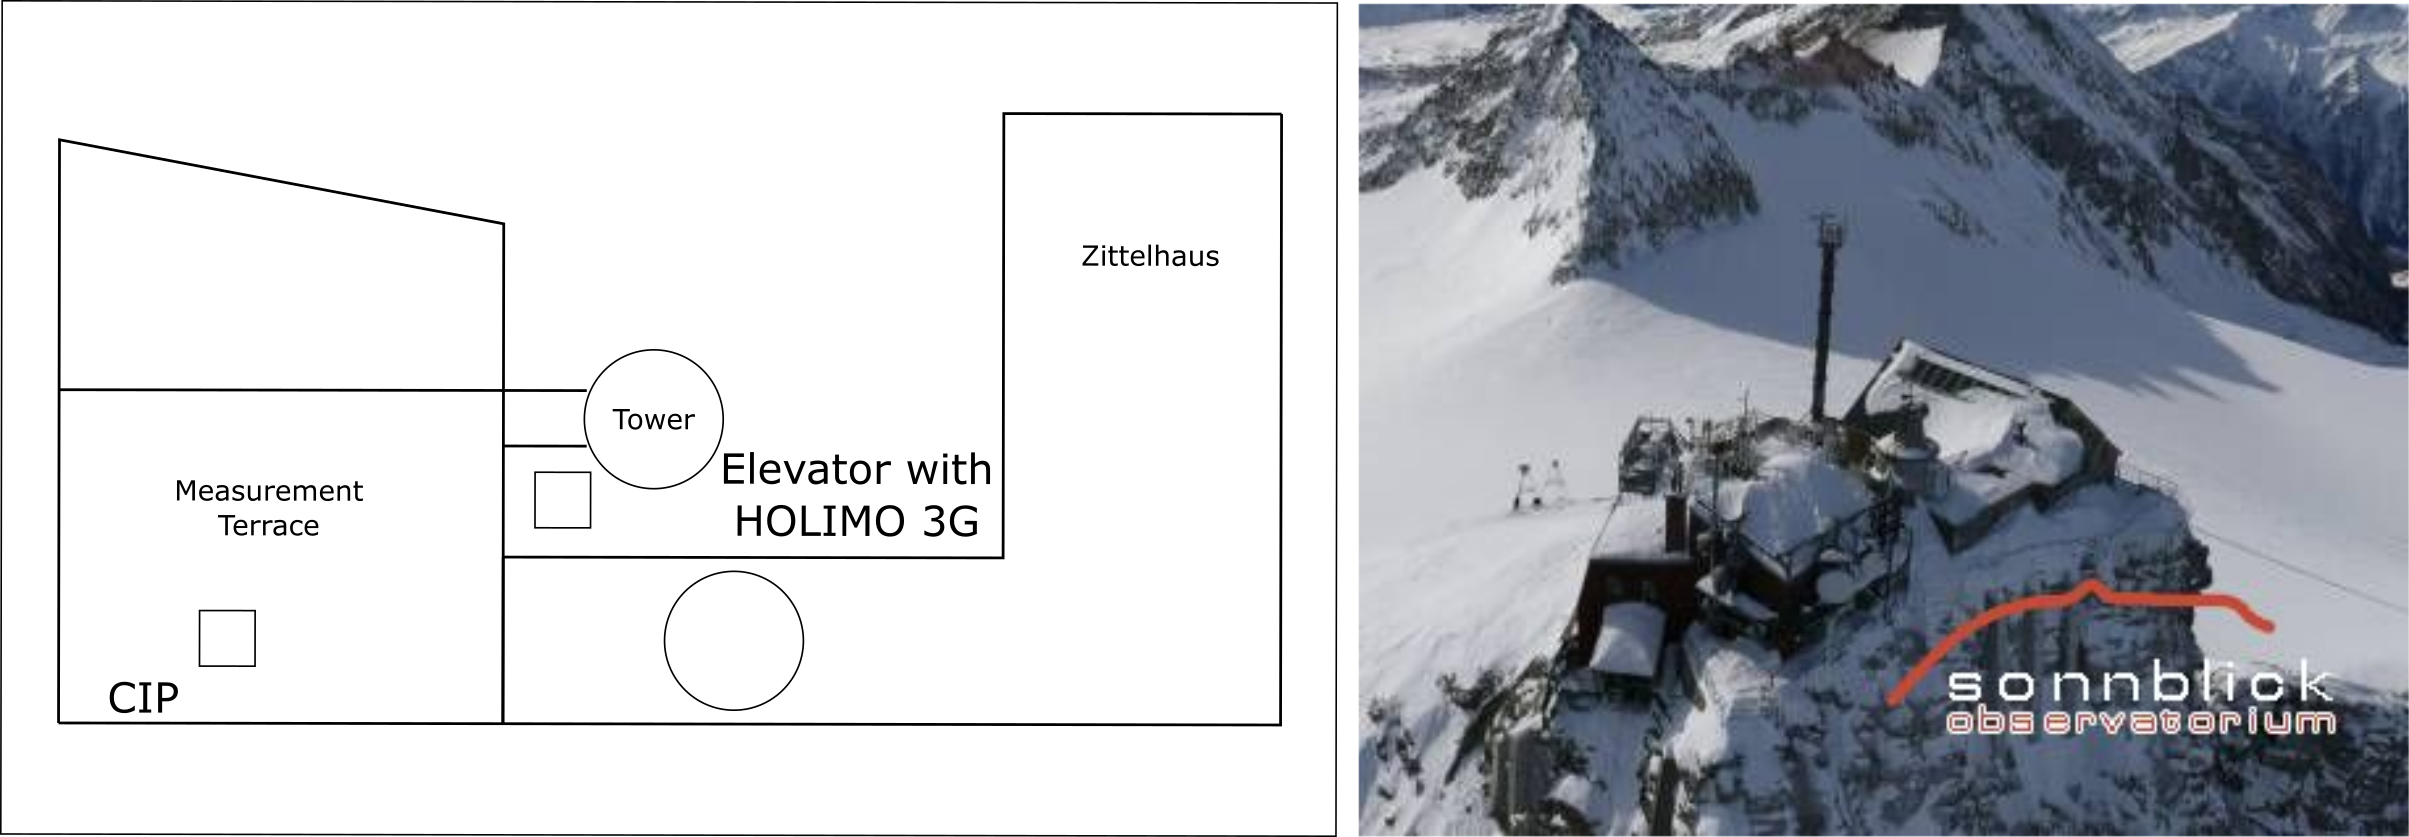
\includegraphics[width=30pc]{SetUp.png}
 \caption{Short caption}
 \label{fig:SetUp}
\end{figure}

\begin{figure}[h]
 \centering
 	\includegraphics[width=10pc]{tower.png}
 \caption{Short caption}
 \label{fig:Elevator}
\end{figure}

\begin{figure}[h]
 \centering
 	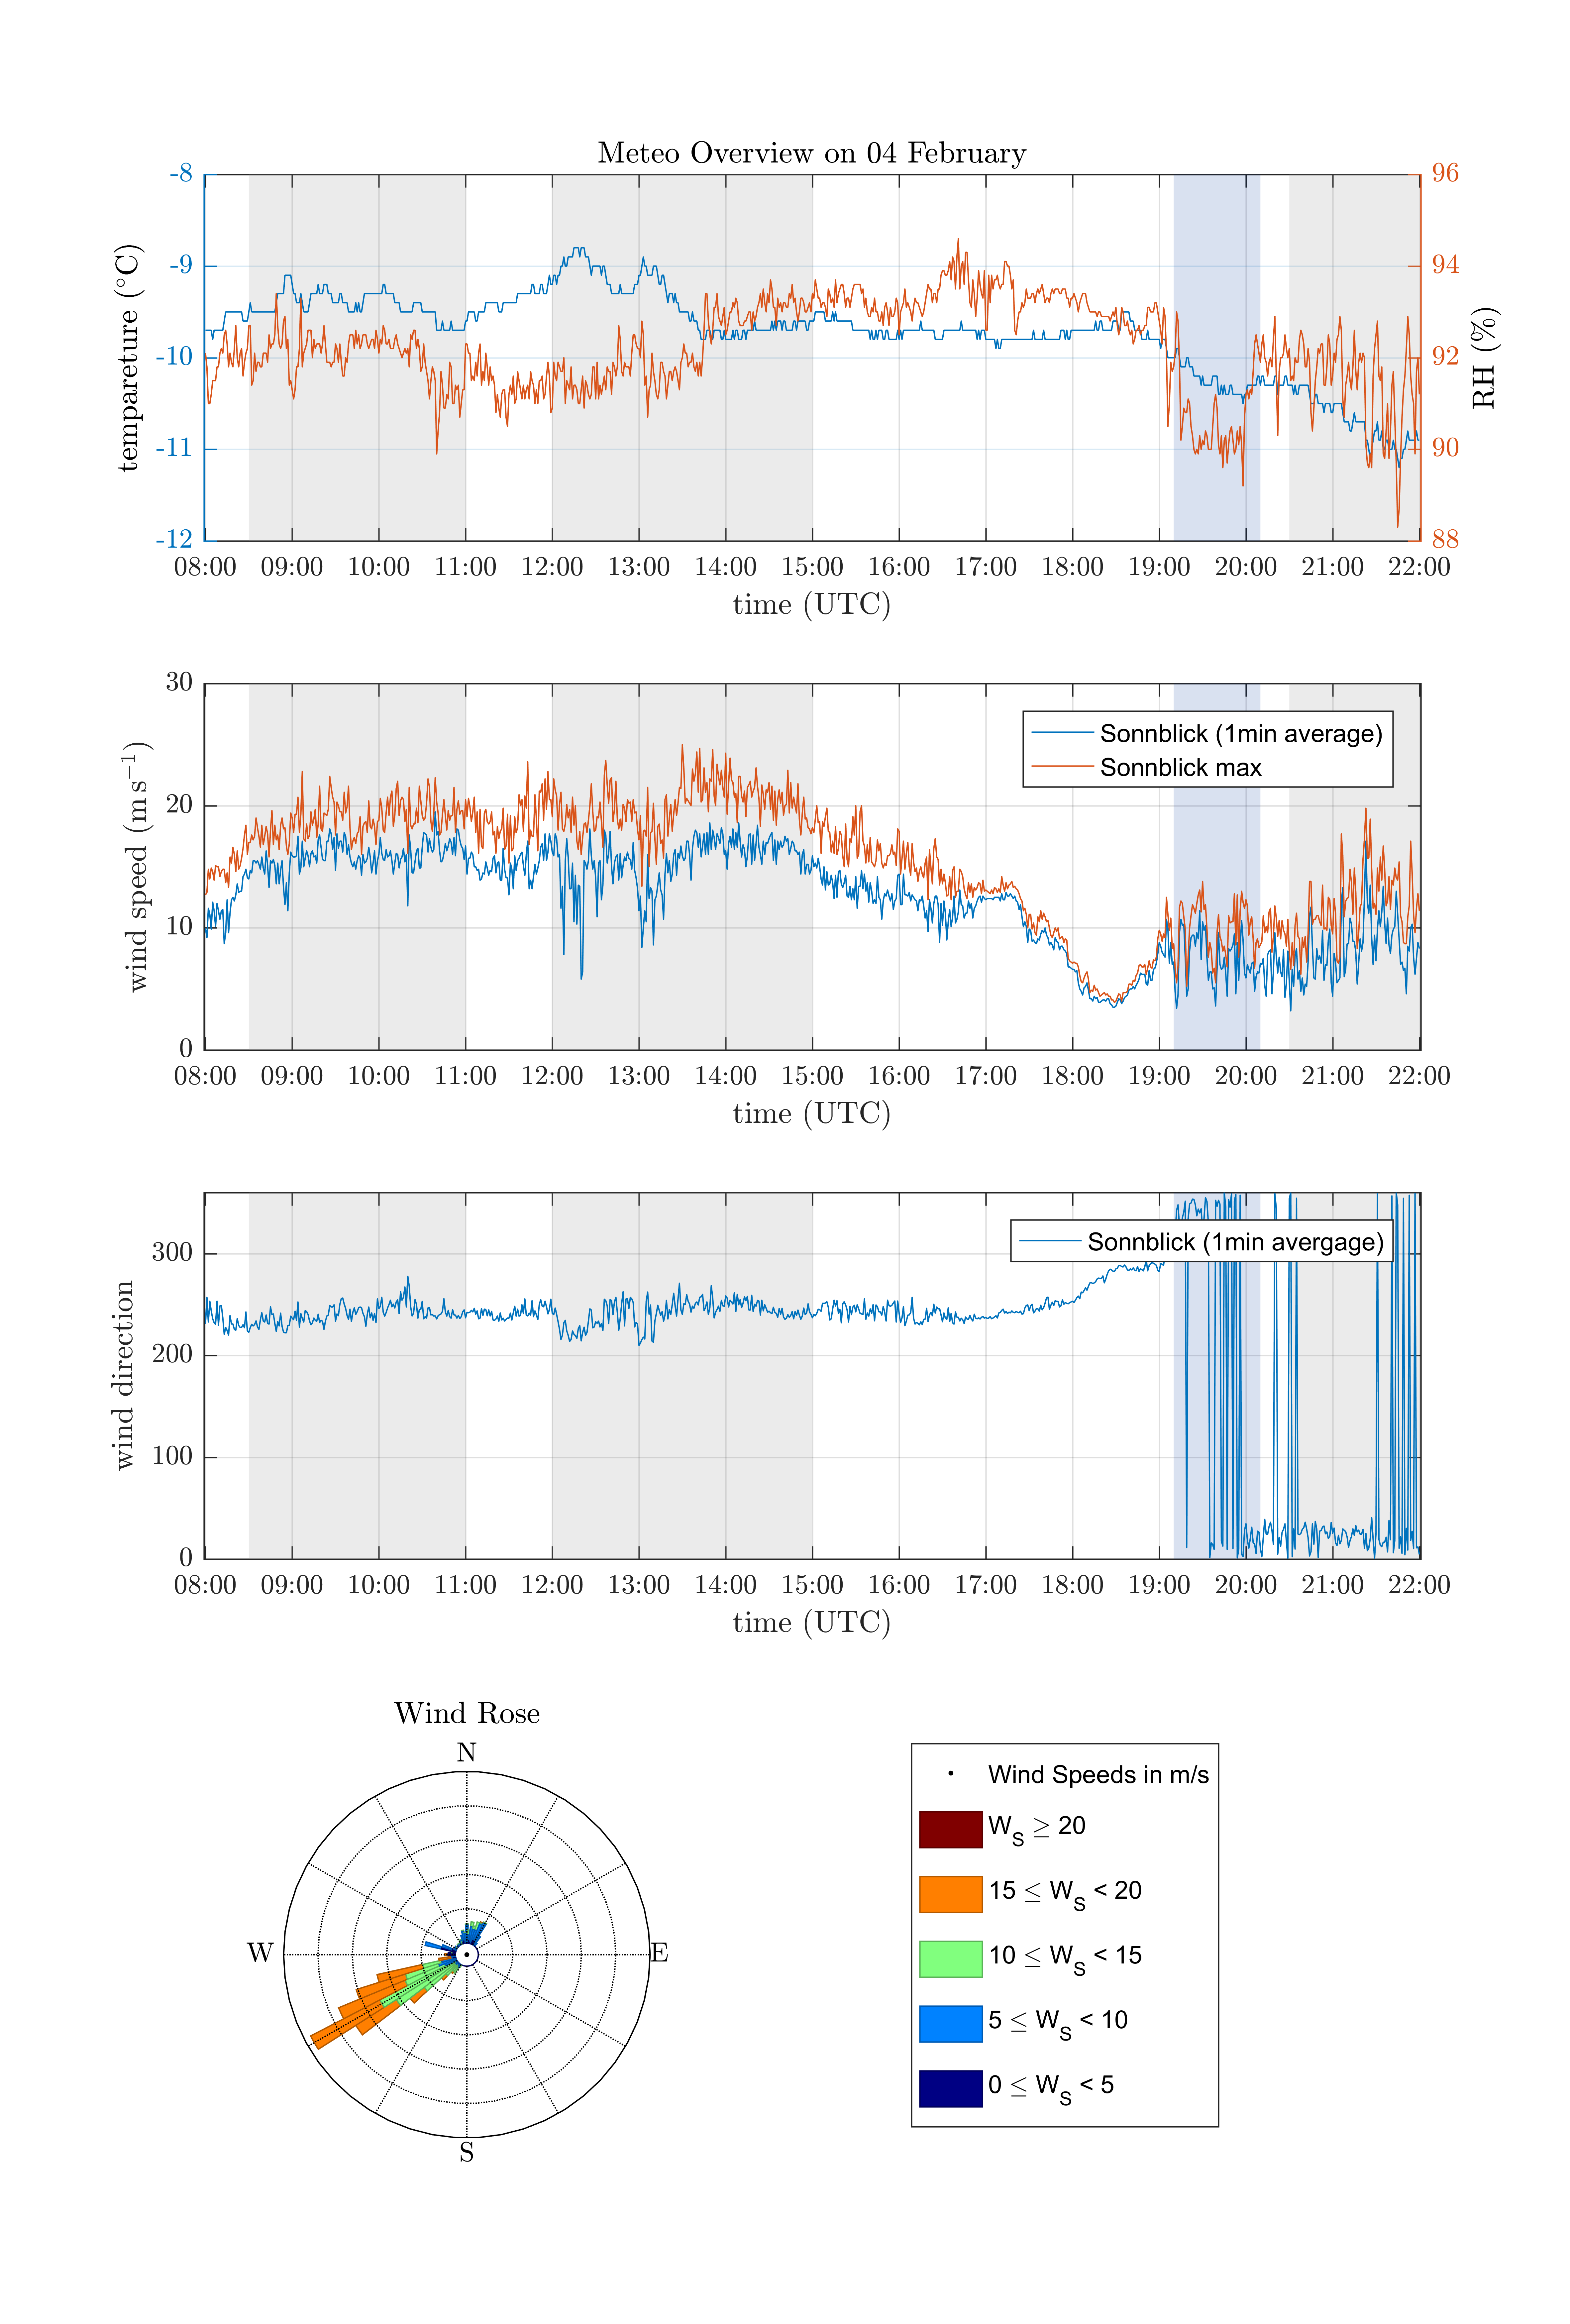
\includegraphics[width=14cm]{MeteoOvervire_0402.png}
 \caption{Overview of the meteorological conditions on 4 February obtained from the SBO measurements. Shown are the temperature, relative humidity (top), wind speed (second from top) and wind direction (second from bottom). All measurements are 1\,\si{m} averages except for the maximum wind speed, which corresponds to the maximum wind speed observed during a corresponding 1\,\si{min} average. A wind rose plot (bottom) of the wind measurement is also shown.}
 \label{fig:meteo0402}
\end{figure}

\begin{figure}[h]
 \centering
 	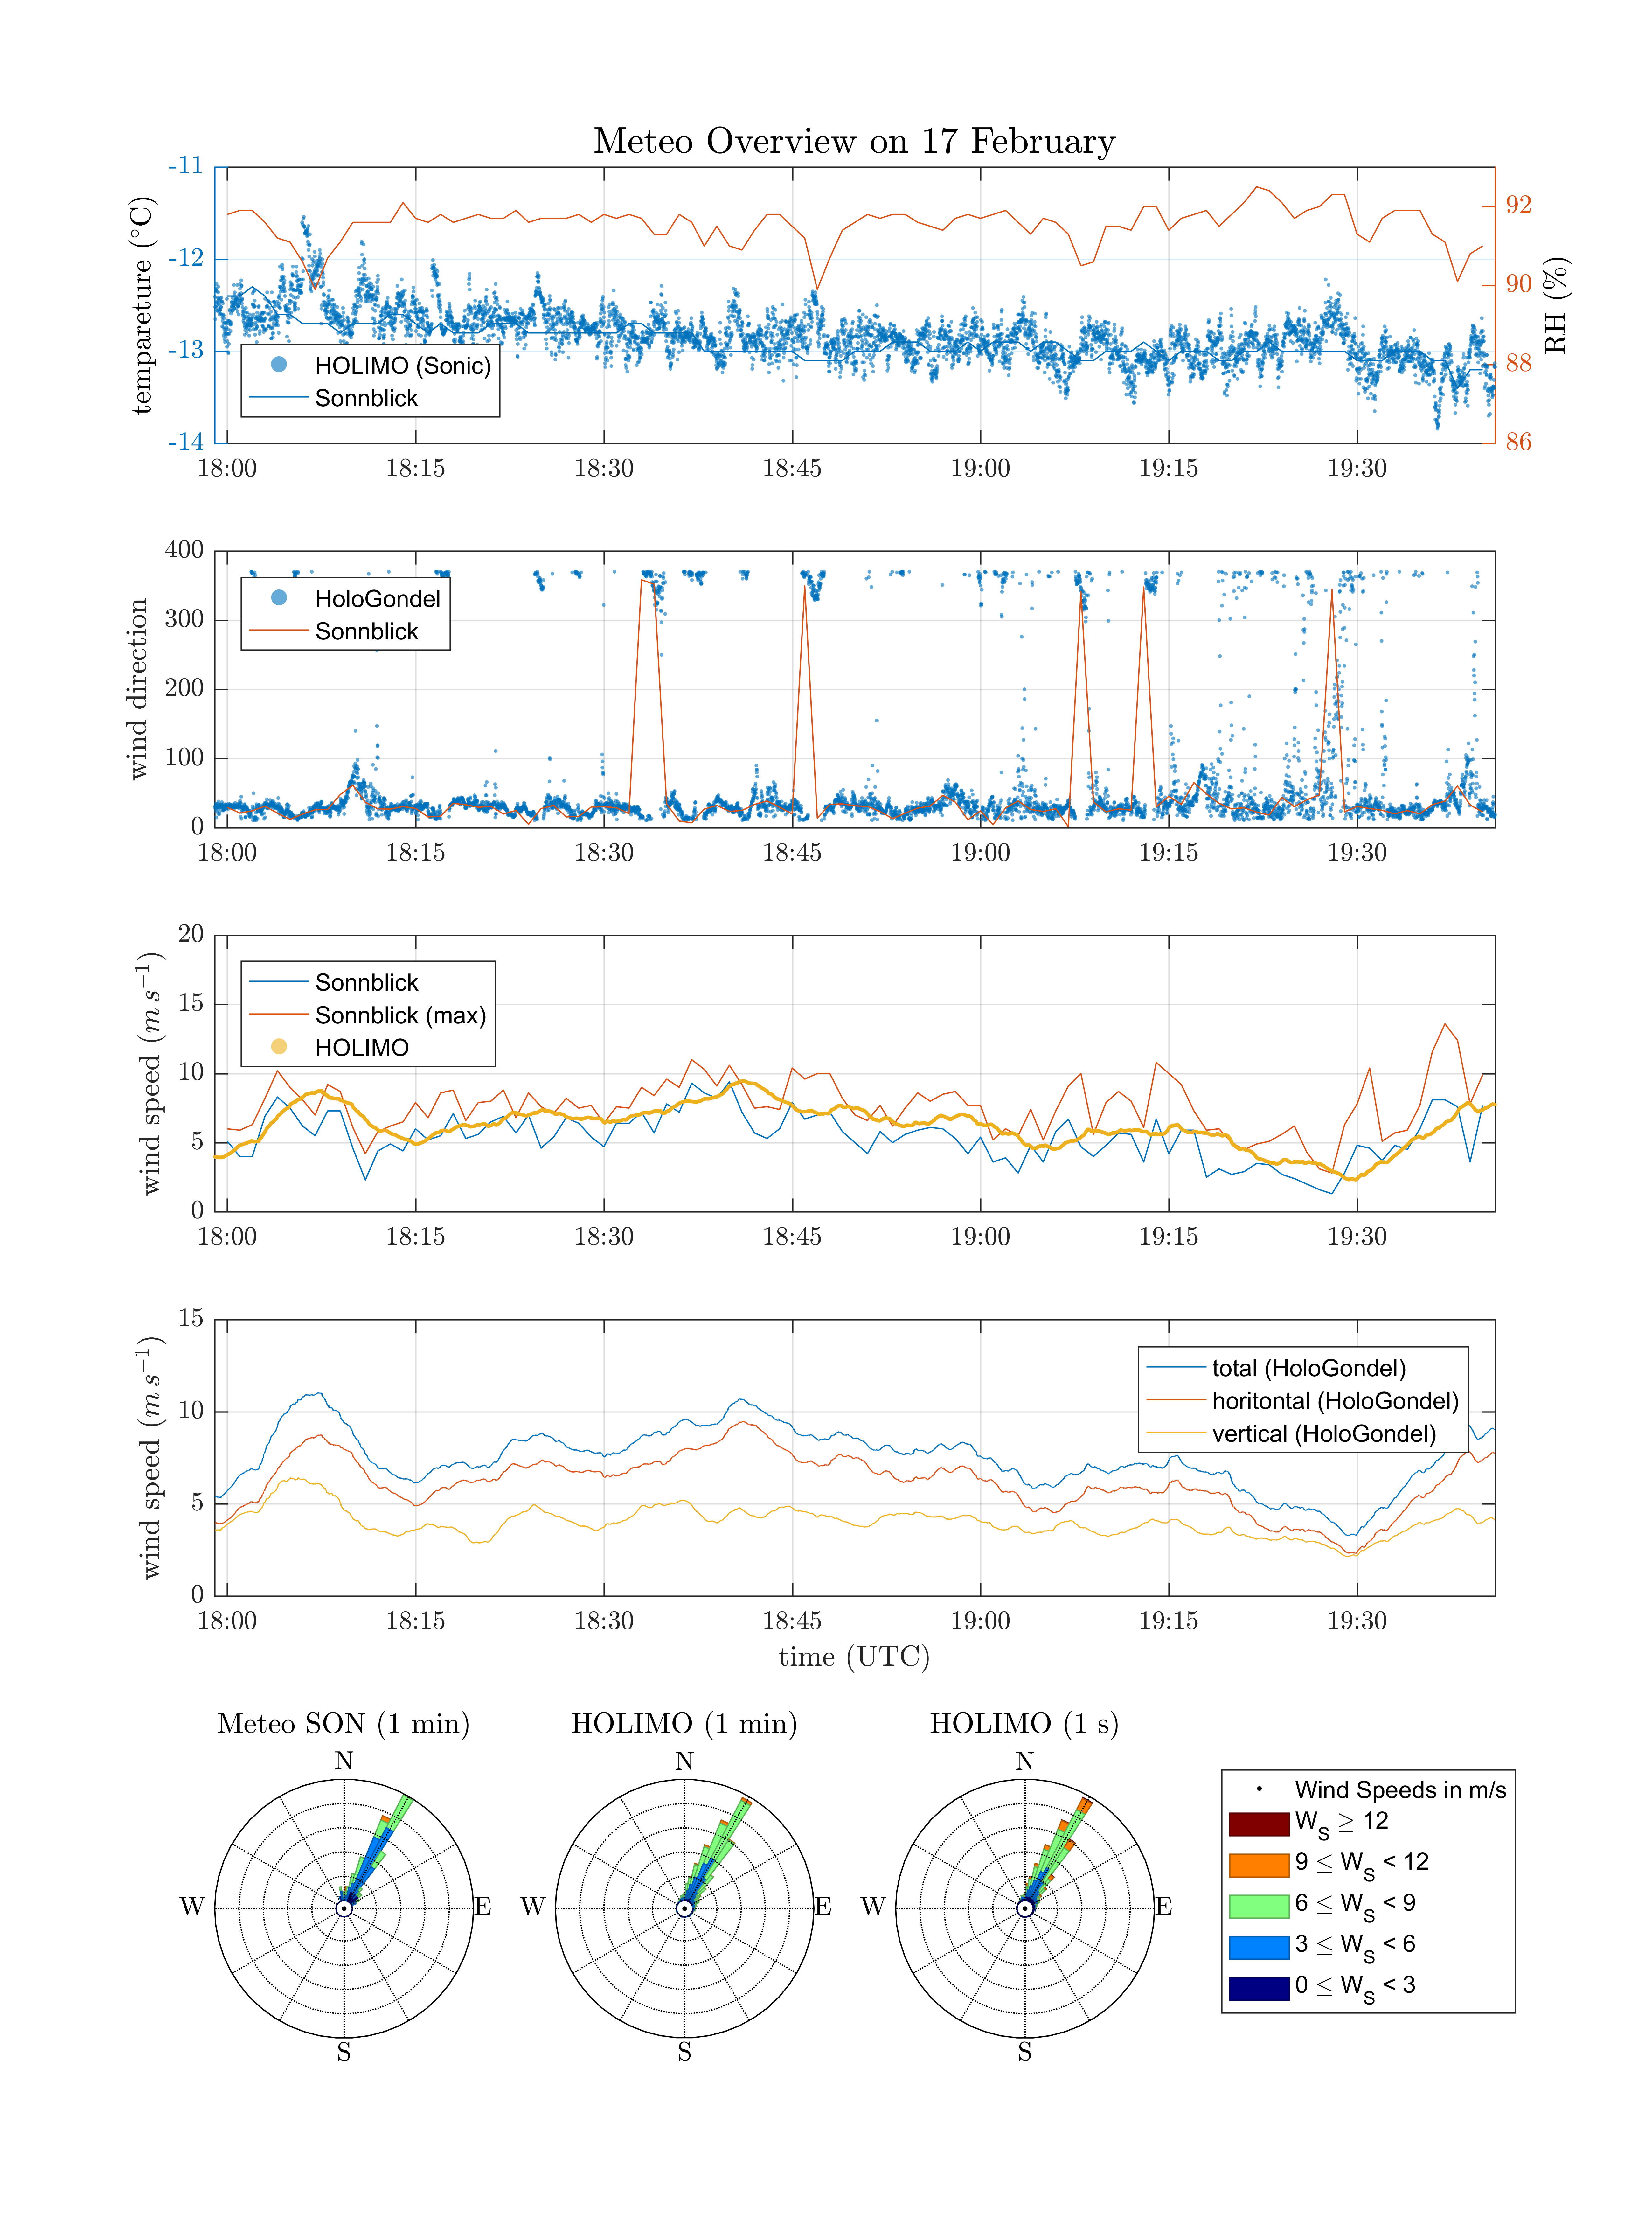
\includegraphics[width=14cm]{MeteoOverview_1702.png}
 \caption{Overview on the meteorological conditions on 17 February. On this day temperature and wind measurements are available from the SBO and the HoloGondel platform. Shown are the temperature (HoloGondel and SBO), relative humidity (top), wind direction (second from top), a comparison of the horizontal wind speed (middle) and detailed wind speed measurements from the HoloGondel platform (second from bottom). A windrose plot is shown in the bottom panel. Wind measurements from the SBO and the HoloGondel platform agree well in direction and velocity.}
 \label{fig:meteo1702}
\end{figure}

\begin{figure}[h]
 \centering
 	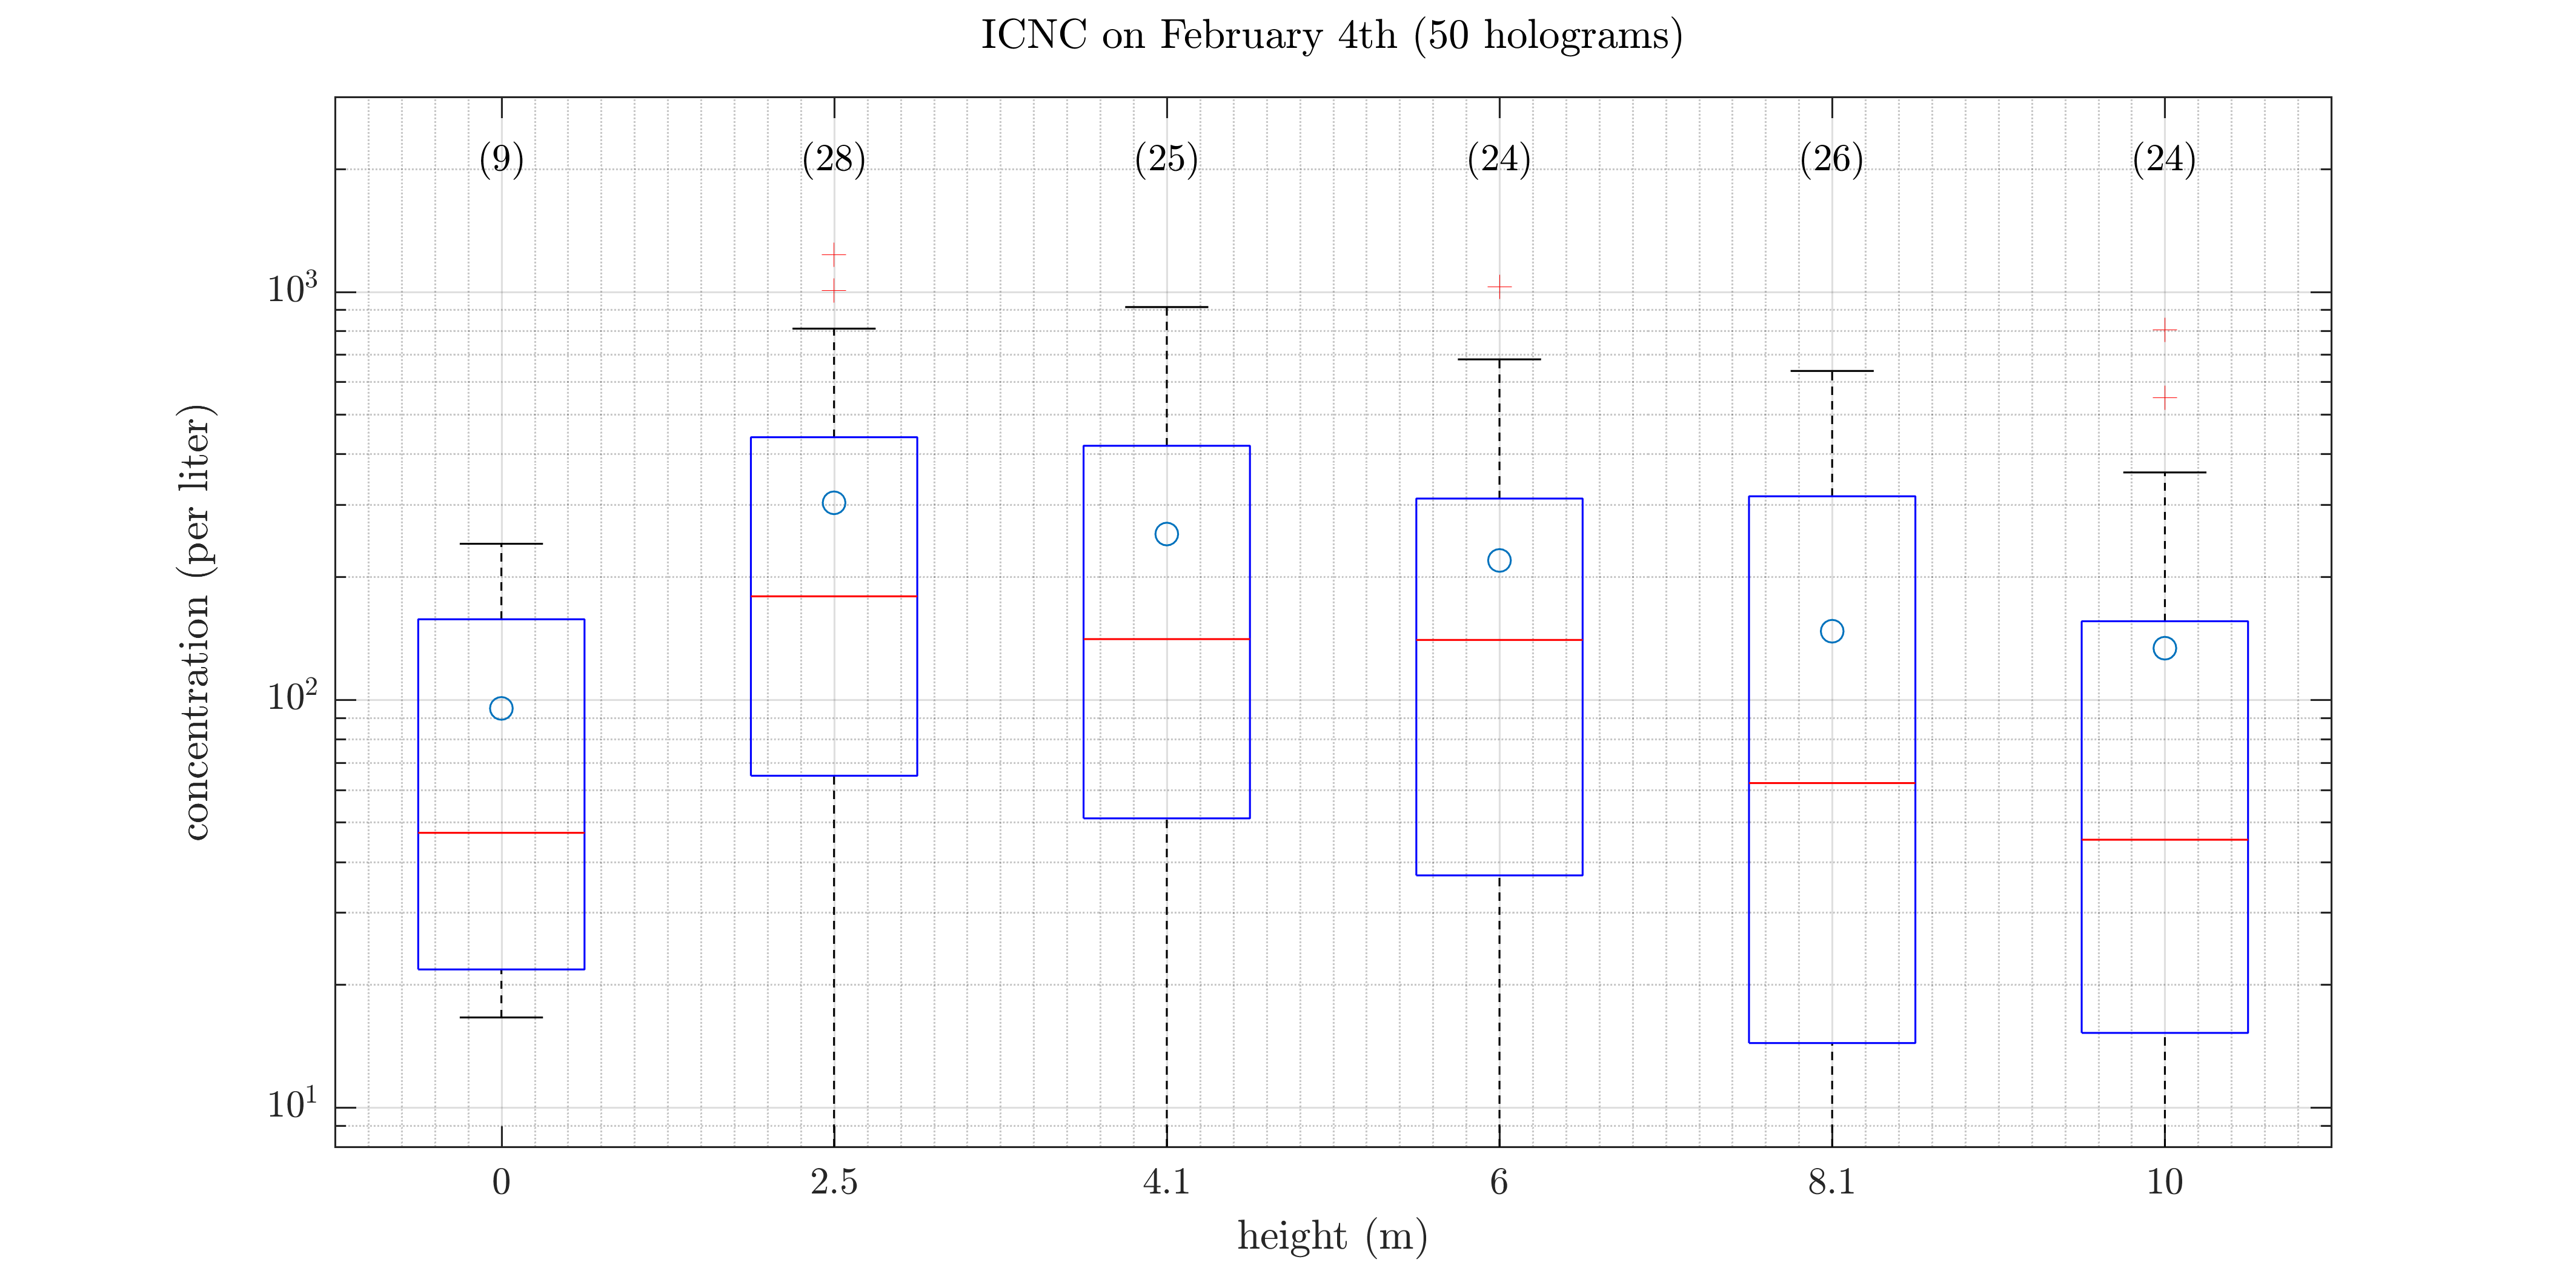
\includegraphics[width=14cm]{0402_Total.png}
 \caption{Ice crystal number concentration as a function of the height of the elevator at the meteorological tower of the SBO. This plot is a summary of the 24 profiles obtained on 4 February. The data was averaged over the entire time period of single measurements at the different height. The number in brackets is the number of measurements points, i.e. the number of measurements, at the different heights. For each box, the central line marks the median value of the measurement and the left and right edges of the box represent 25th and the 75th percentiles respectively. The whiskers extend to minimum and maximum of the data; outliers are marked as red pluses. The mean value of the measurements is indicated as a blue circle.}
 \label{fig:Total0402}
\end{figure}

\begin{figure}[h]
 \centering
 	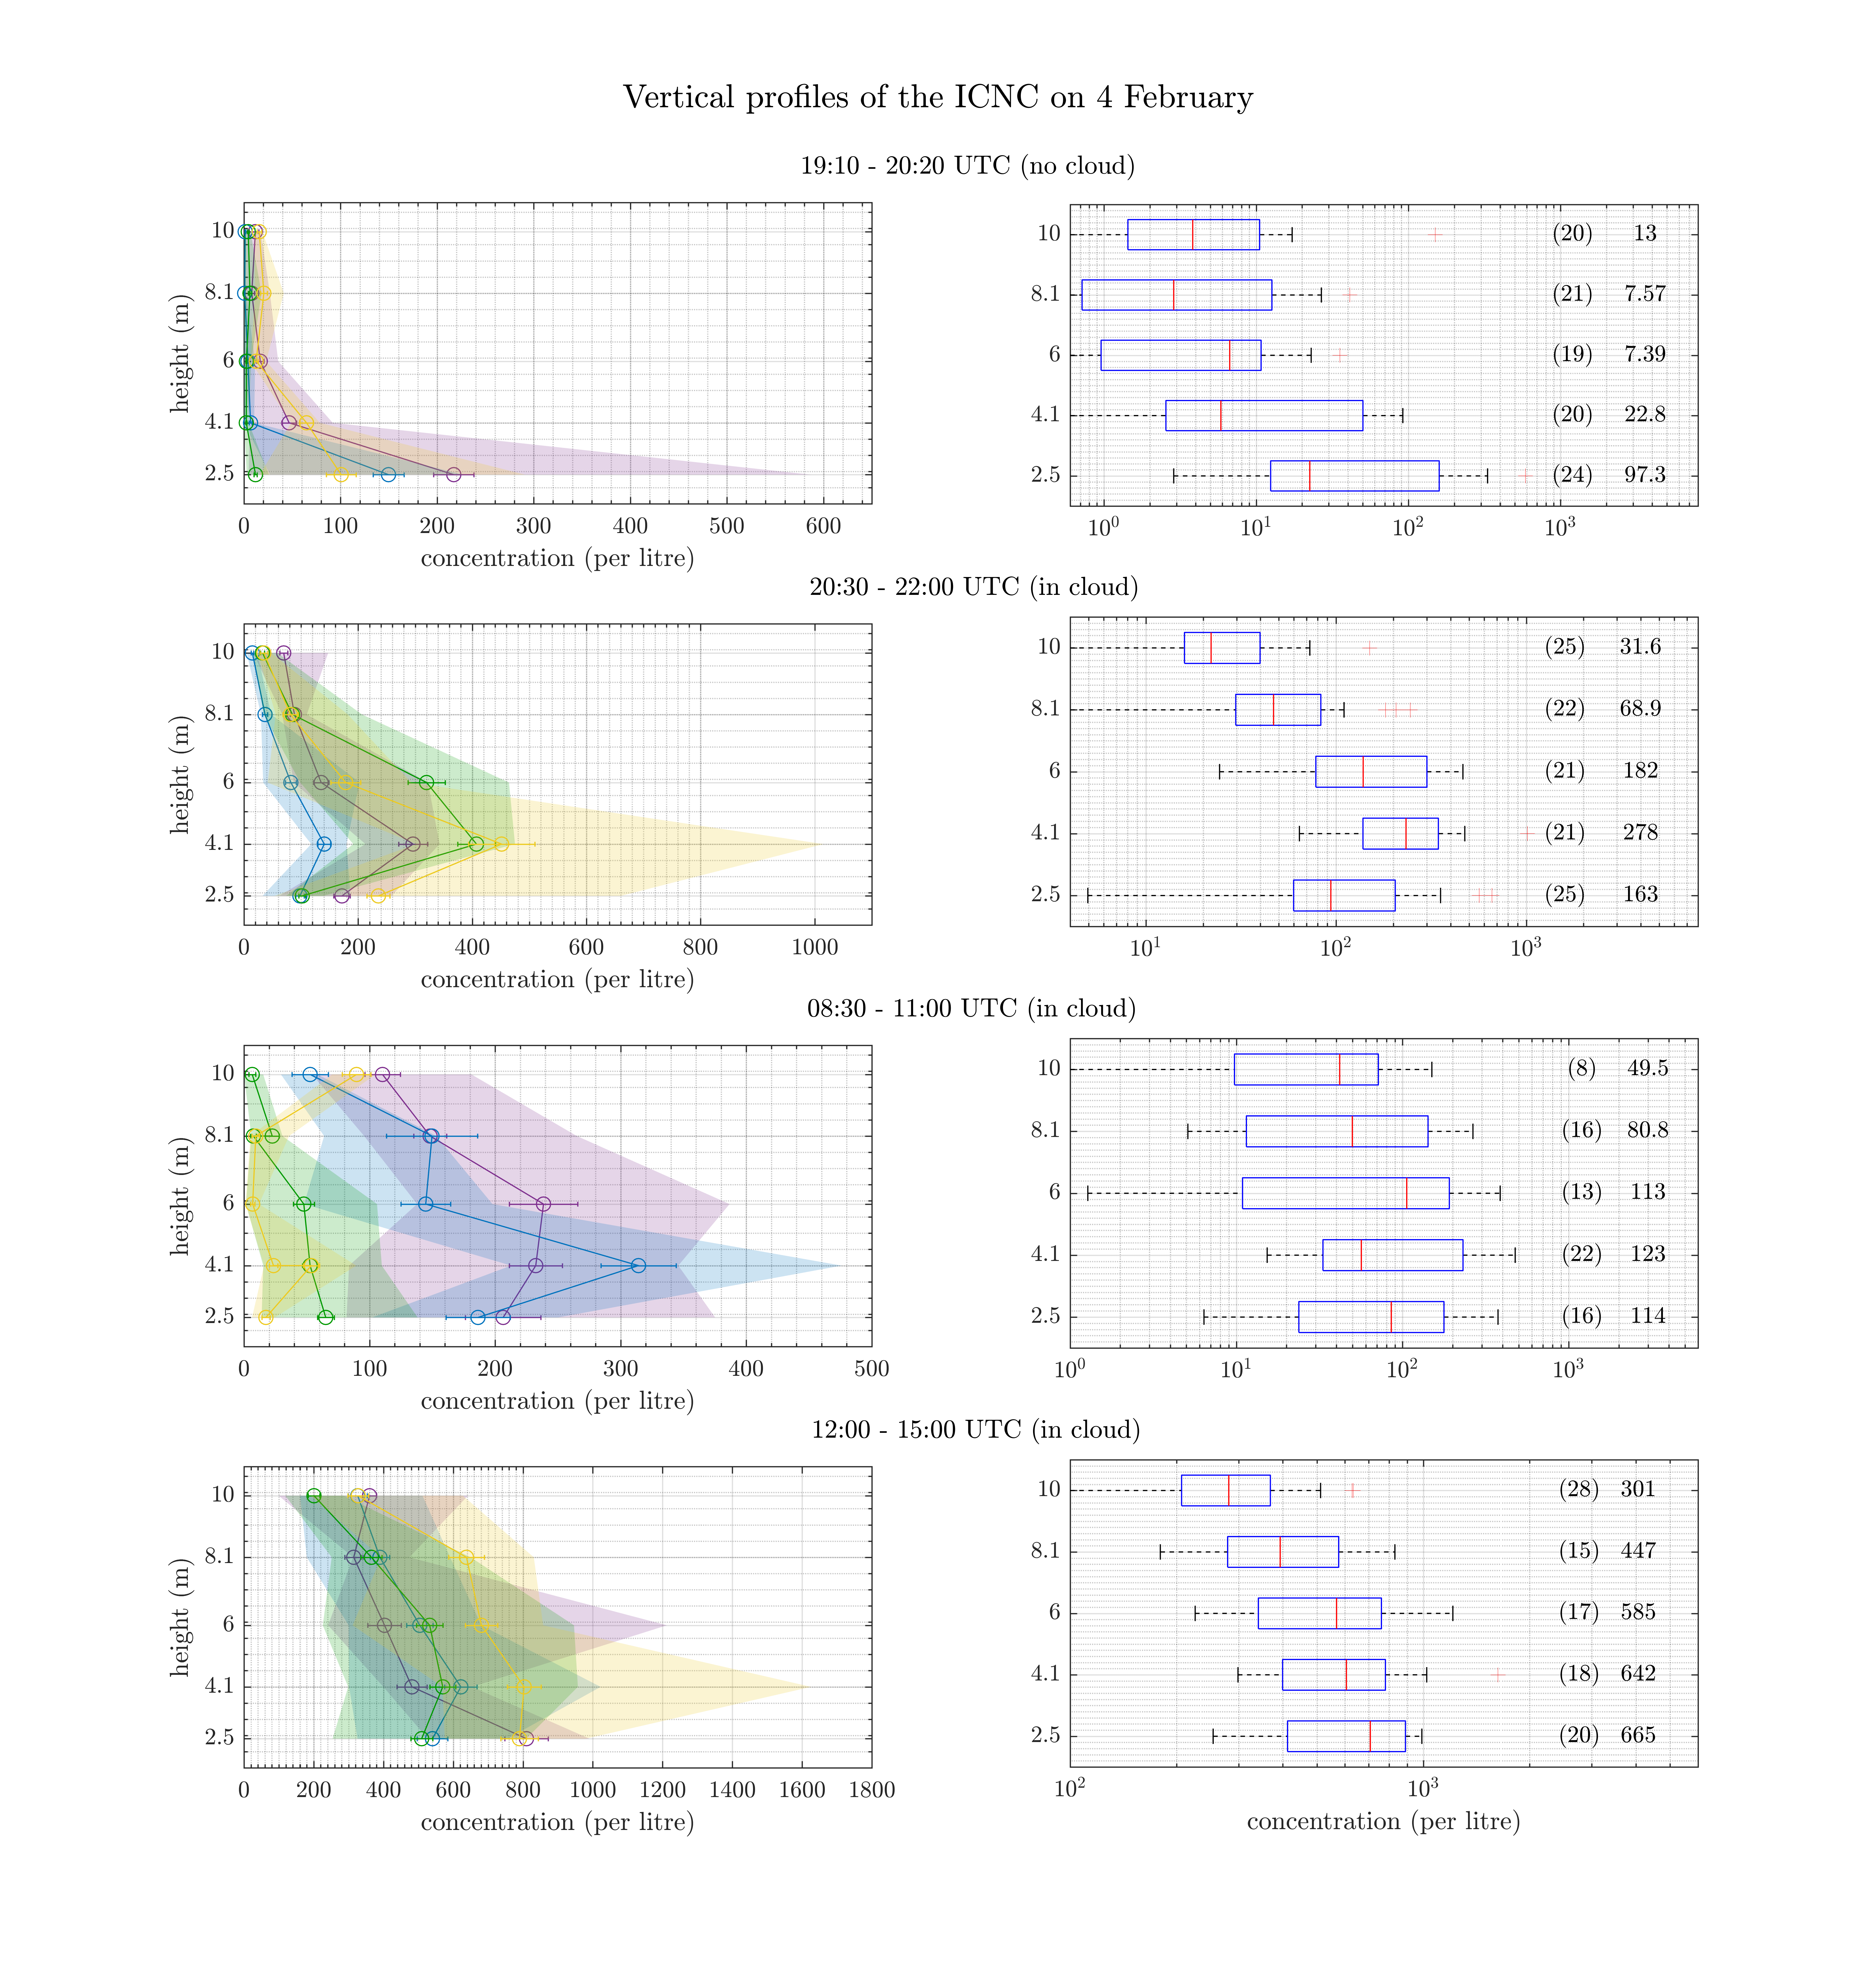
\includegraphics[width=14cm]{0402_Overview.png}
 \caption{Ice crystal number concentration as a function of the height of the elevator at the meteorological tower of the SBO for four different timer intervals during 4 February, representing different meteorological conditions (Fig. \ref{fig:meteo0402}). The individual profiles (left) are a representation for the different time intervals. The circles indicate the mean value averaged over the entire time interval. The error bars represent the standard error of the mean. The shaded area indicates the variability of the data and extends from the minimum to the maximum when the data is averaged over 50 holograms. For the summary of the different time intervals (right) the data is averaged over 50 holograms. For each box, the central line marks the median value of the measurement and the left and right edges of the box represent 25th and the 75th percentiles respectively. The whiskers extend to minimum and maximum of the data; outliers are marked as red pluses.}
 \label{fig:profiles0402}
\end{figure}

\begin{figure}[h]
 \centering
 	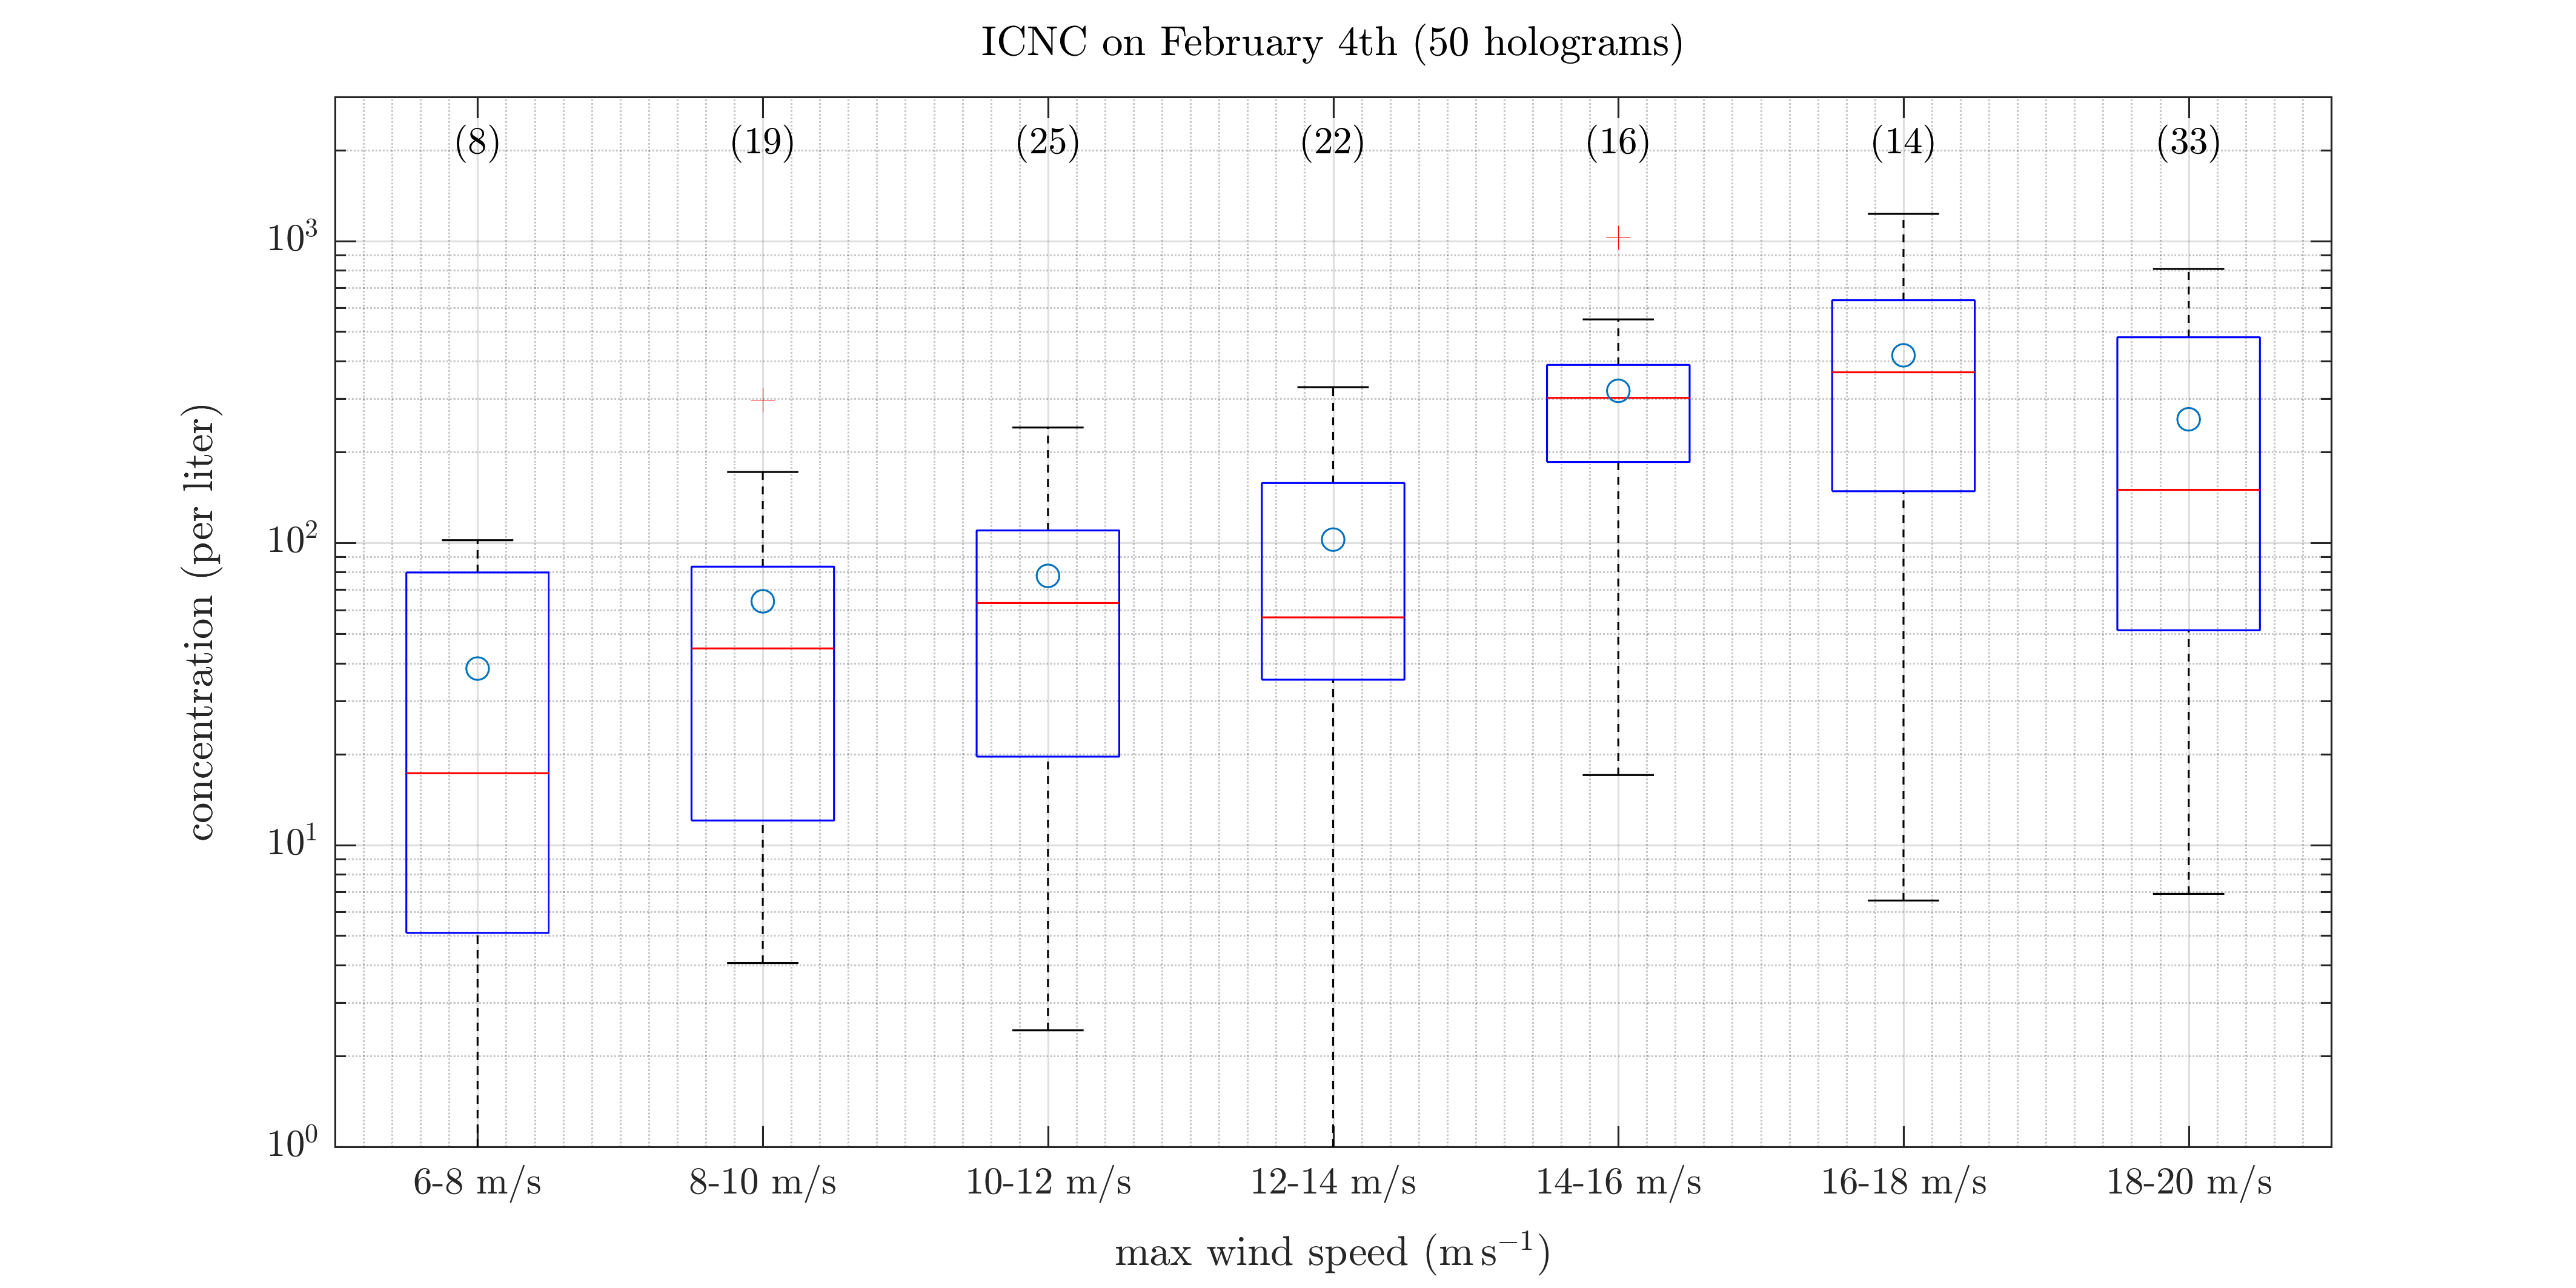
\includegraphics[width=14cm]{0402_WSMax.png}
 \caption{Ice crystal number concentration as a function of vertical wind speed. This plot is a summary of the entire data obtained on 4 February. The data was averaged over 50 holograms and categorized in 2\,\si{m\,s^{-1}} wind speed intervals. The wind speeds are one minute averages from the SBO. The number in brackets is the number of measurements points, i.e. the number of measurements, obtained for the different wind speed intervals. For each box, the central line marks the median value of the measurement and the left and right edges of the box represent 25th and the 75th percentiles respectively. The whiskers extend to minimum and maximum of the data; outliers are marked as red pluses. The mean value of the measurements is indicated as a blue circle.}
 \label{fig:ICNCvsWSMAX0402}
\end{figure}

\begin{figure}[h]
 \centering
 	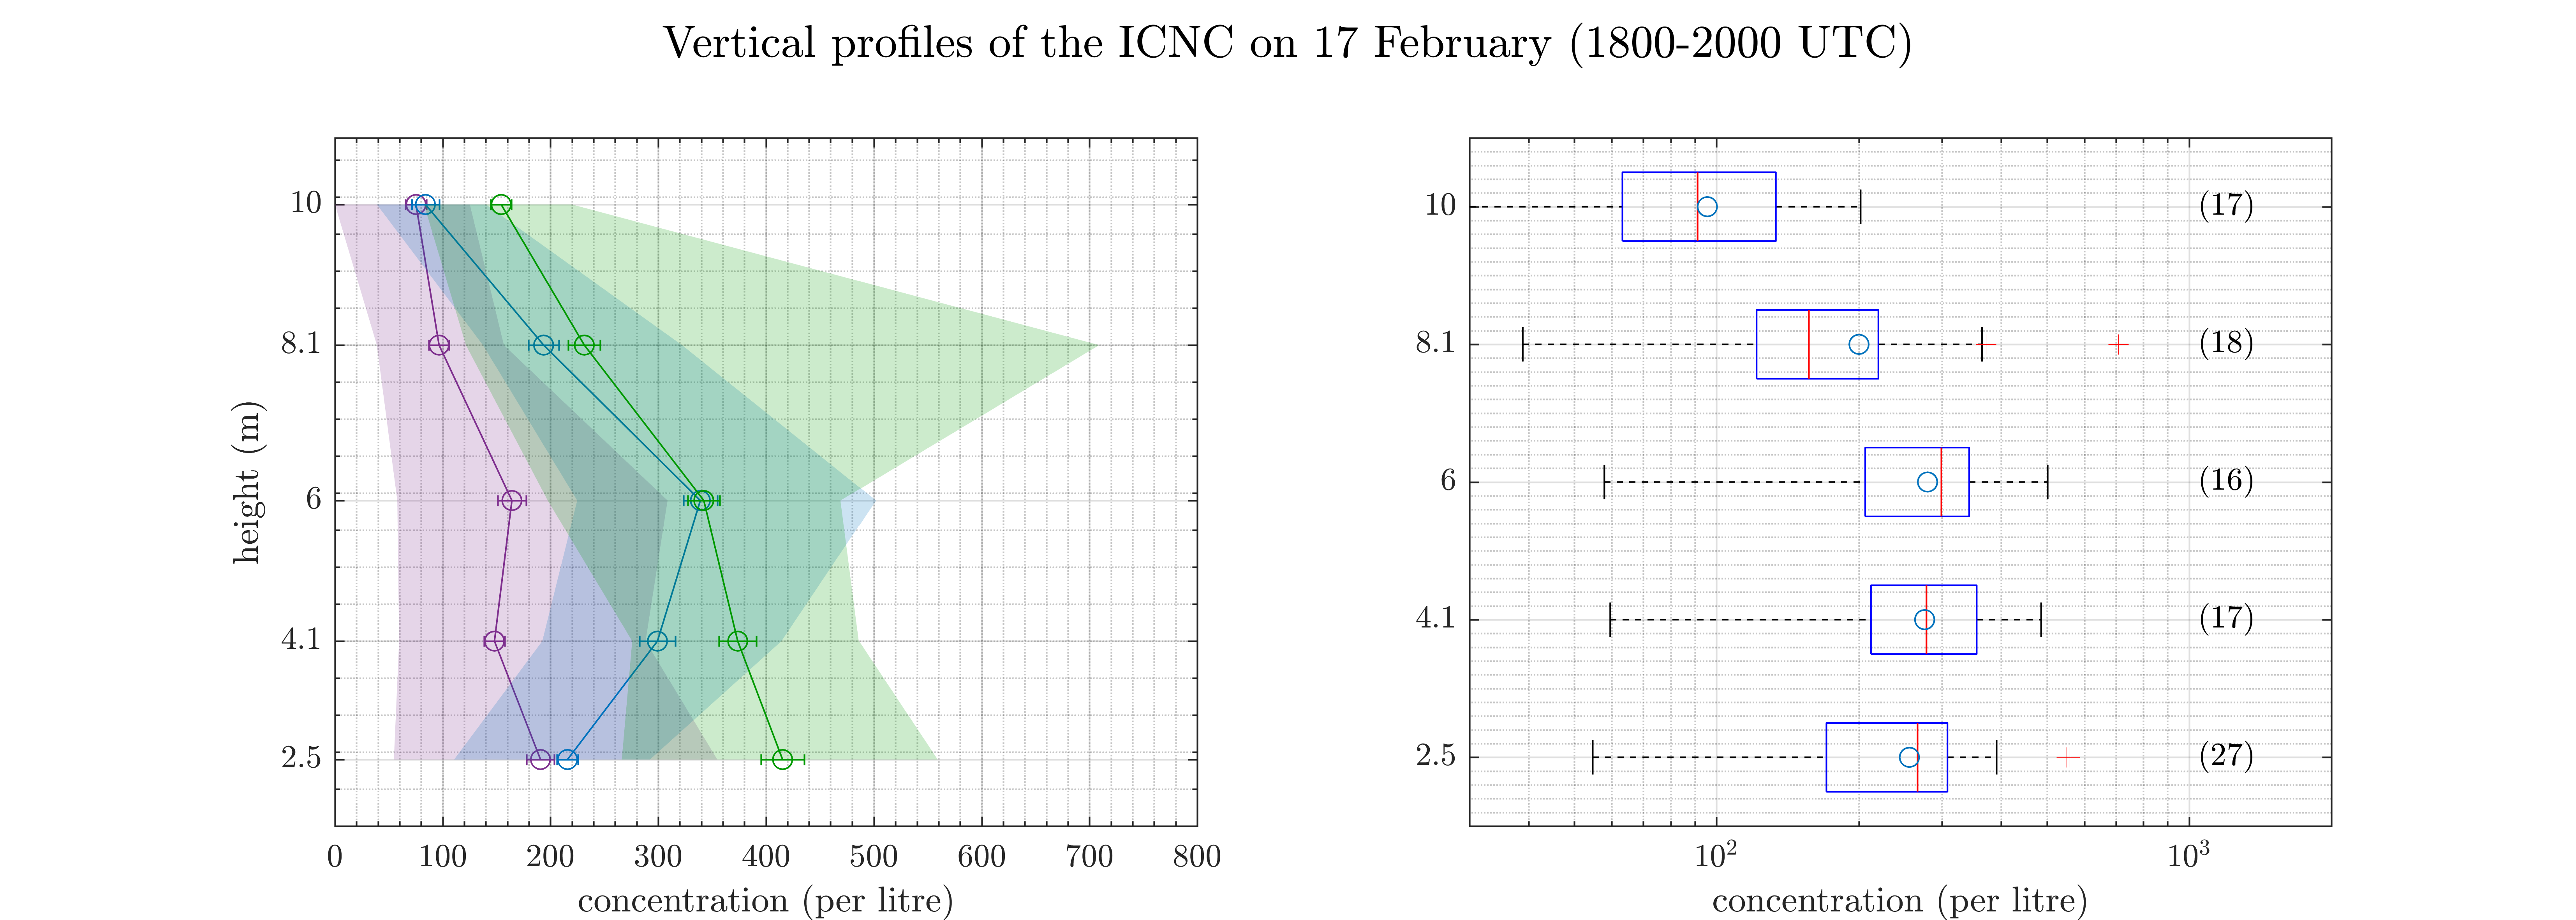
\includegraphics[width=14cm]{1702_Overview.png}
 \caption{Ice crystal number concentration as a function of the height of the elevator at the meteorological tower of the SBO for 17 February. On the left are the three individual profiles obtained in cloud. The circles indicate the mean value averaged over the entire time interval. The error bars represent the standard error of the mean. The shaded area indicates the variability of the data and extends from the minimum to the maximum when the data is averaged over 50 holograms. For the summary of the different time intervals (right) the data is averaged over 50 holograms. For each box, the central line marks the median value of the measurement and the left and right edges of the box represent 25th and the 75th percentiles respectively. The whiskers extend to minimum and maximum of the data; outliers are marked as red pluses.}
 \label{fig:profiles1702}
\end{figure}

\begin{figure}[h]
 \centering
 	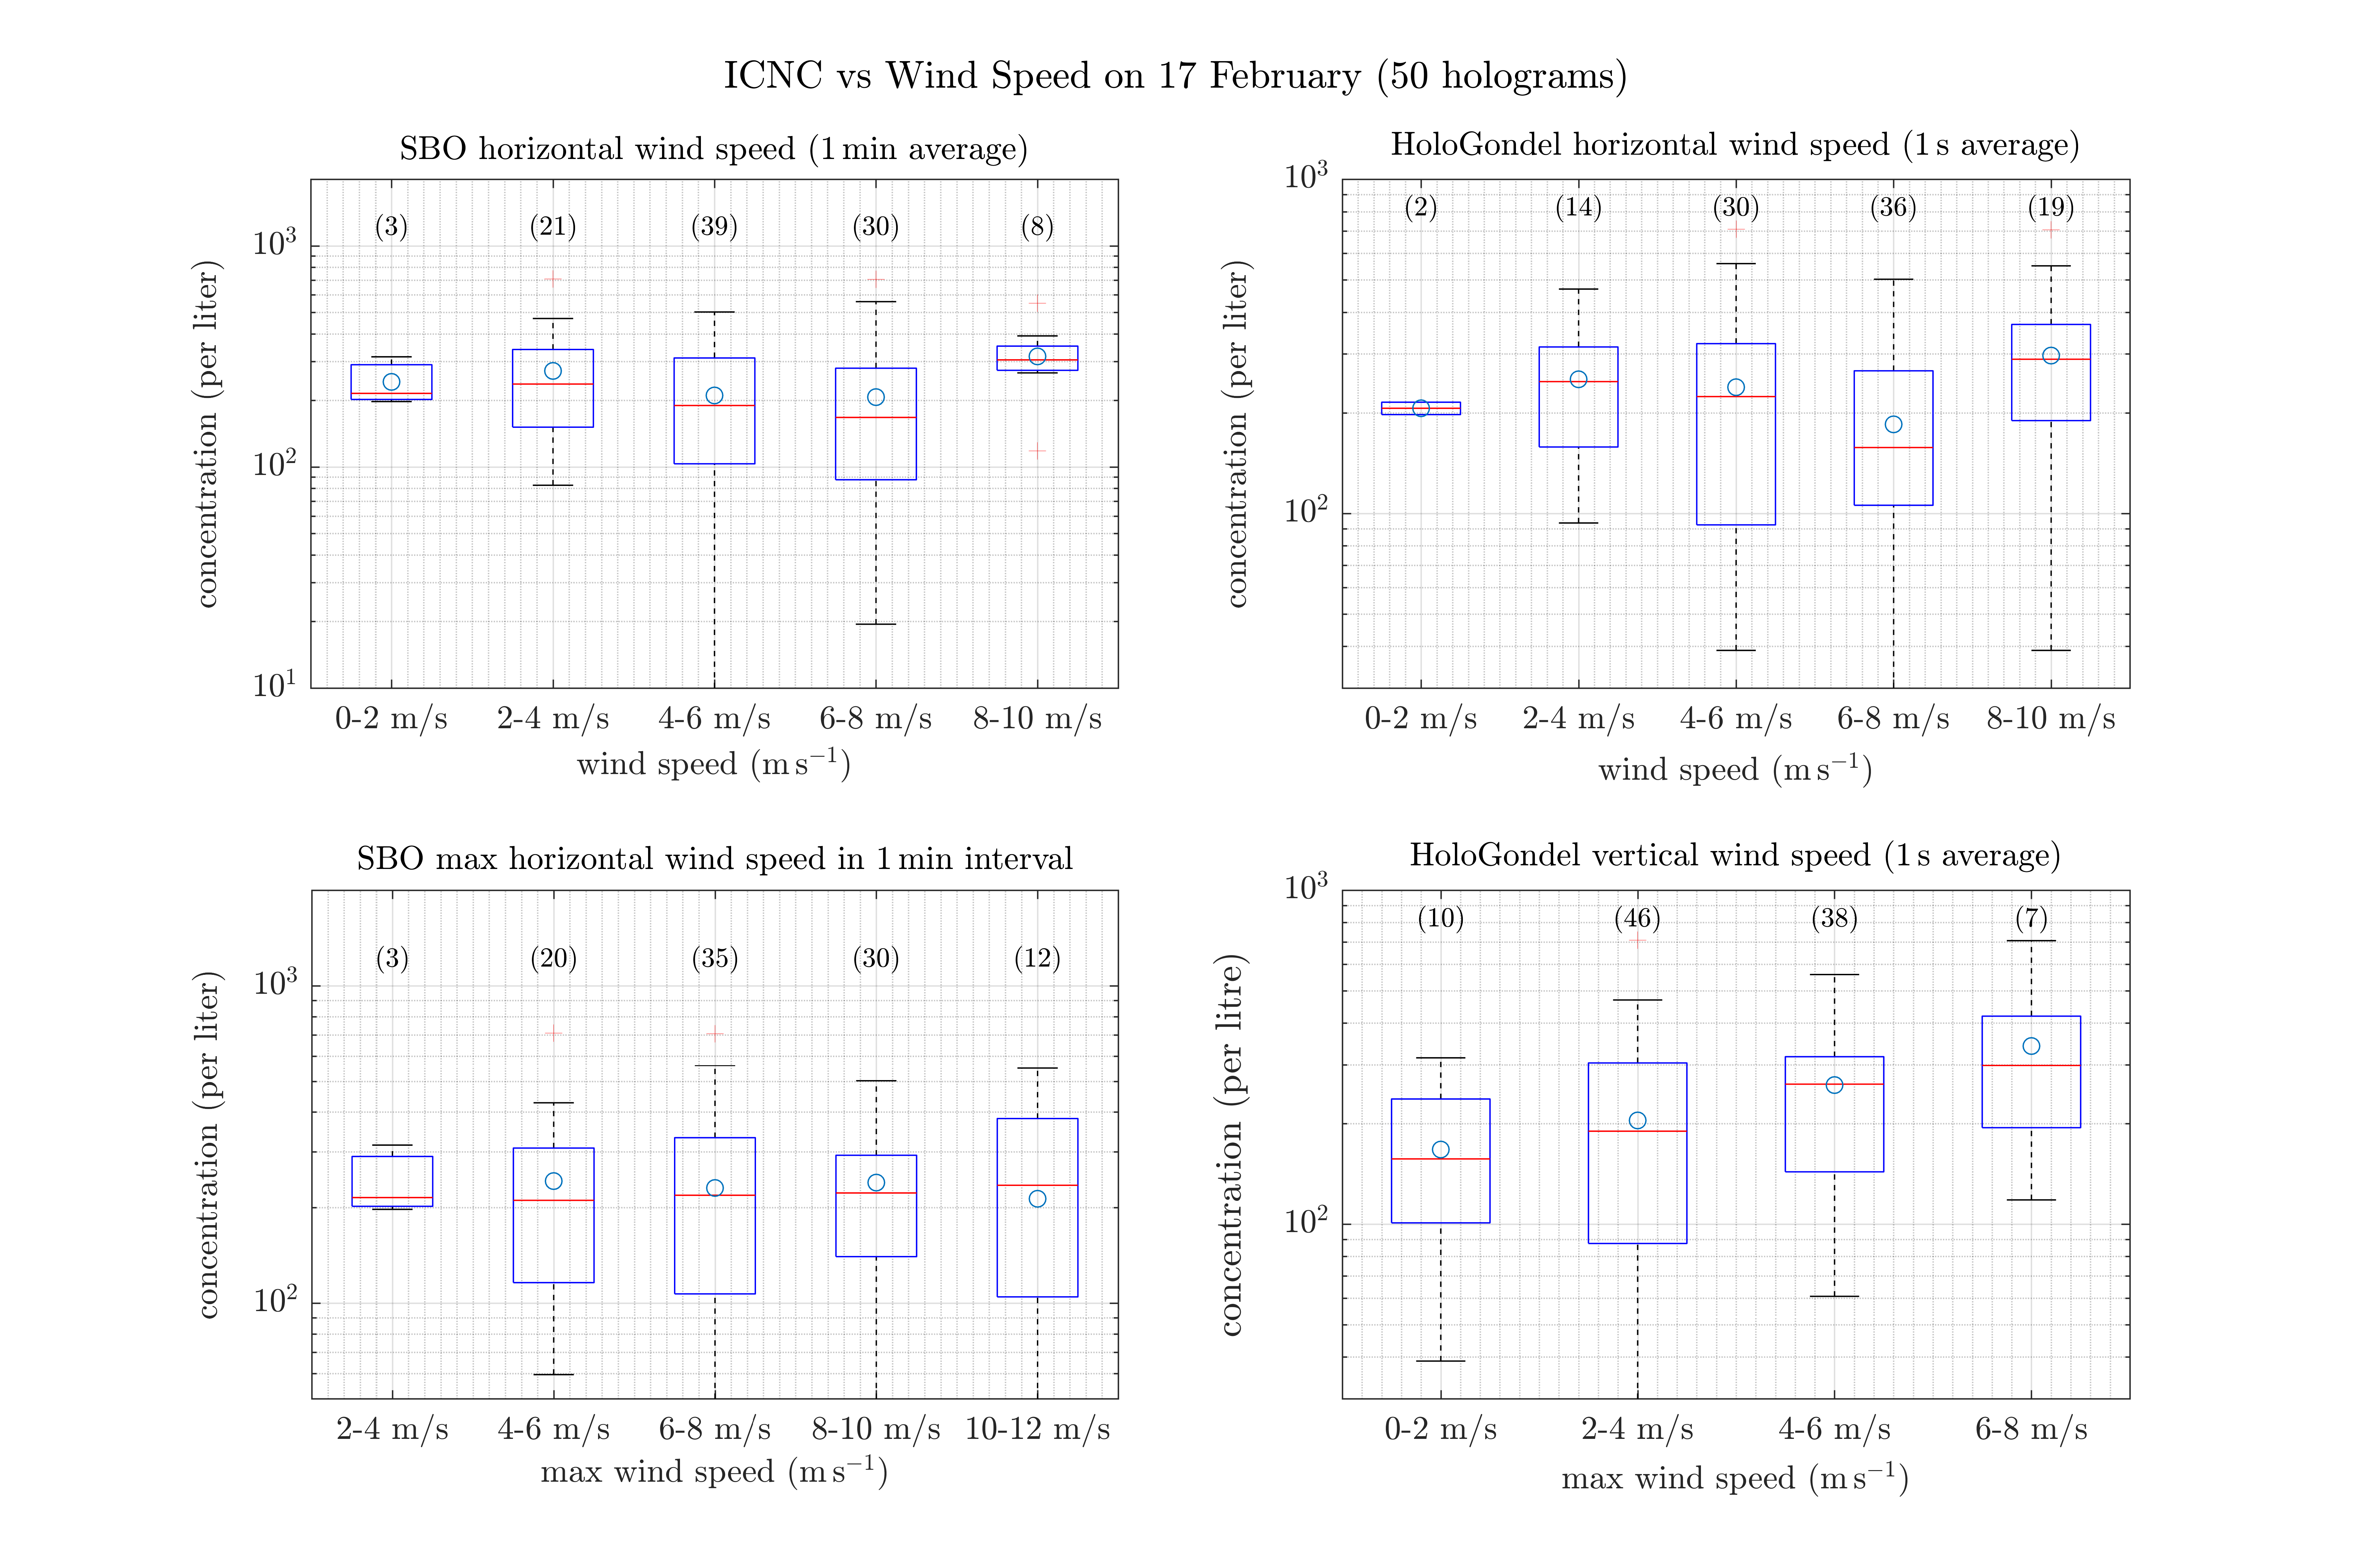
\includegraphics[width=14cm]{1702_OverviewWS.png}
 \caption{As Figure \ref{fig:ICNCvsWSMAX0402} only for 17 February and four different wind speed measurements: a) one minute averages of the horizontal wind speed from the SBO, b) maximum wind speed of the a corresponding time interval in a), c) secondly averages of the horizontal wind speed and d) secondly average of the vertical wind speed both from the 3D Sonic Anemometer.}
 \label{fig:ICNCvsWind1702}
\end{figure}

\begin{figure}[h]
 \centering
 	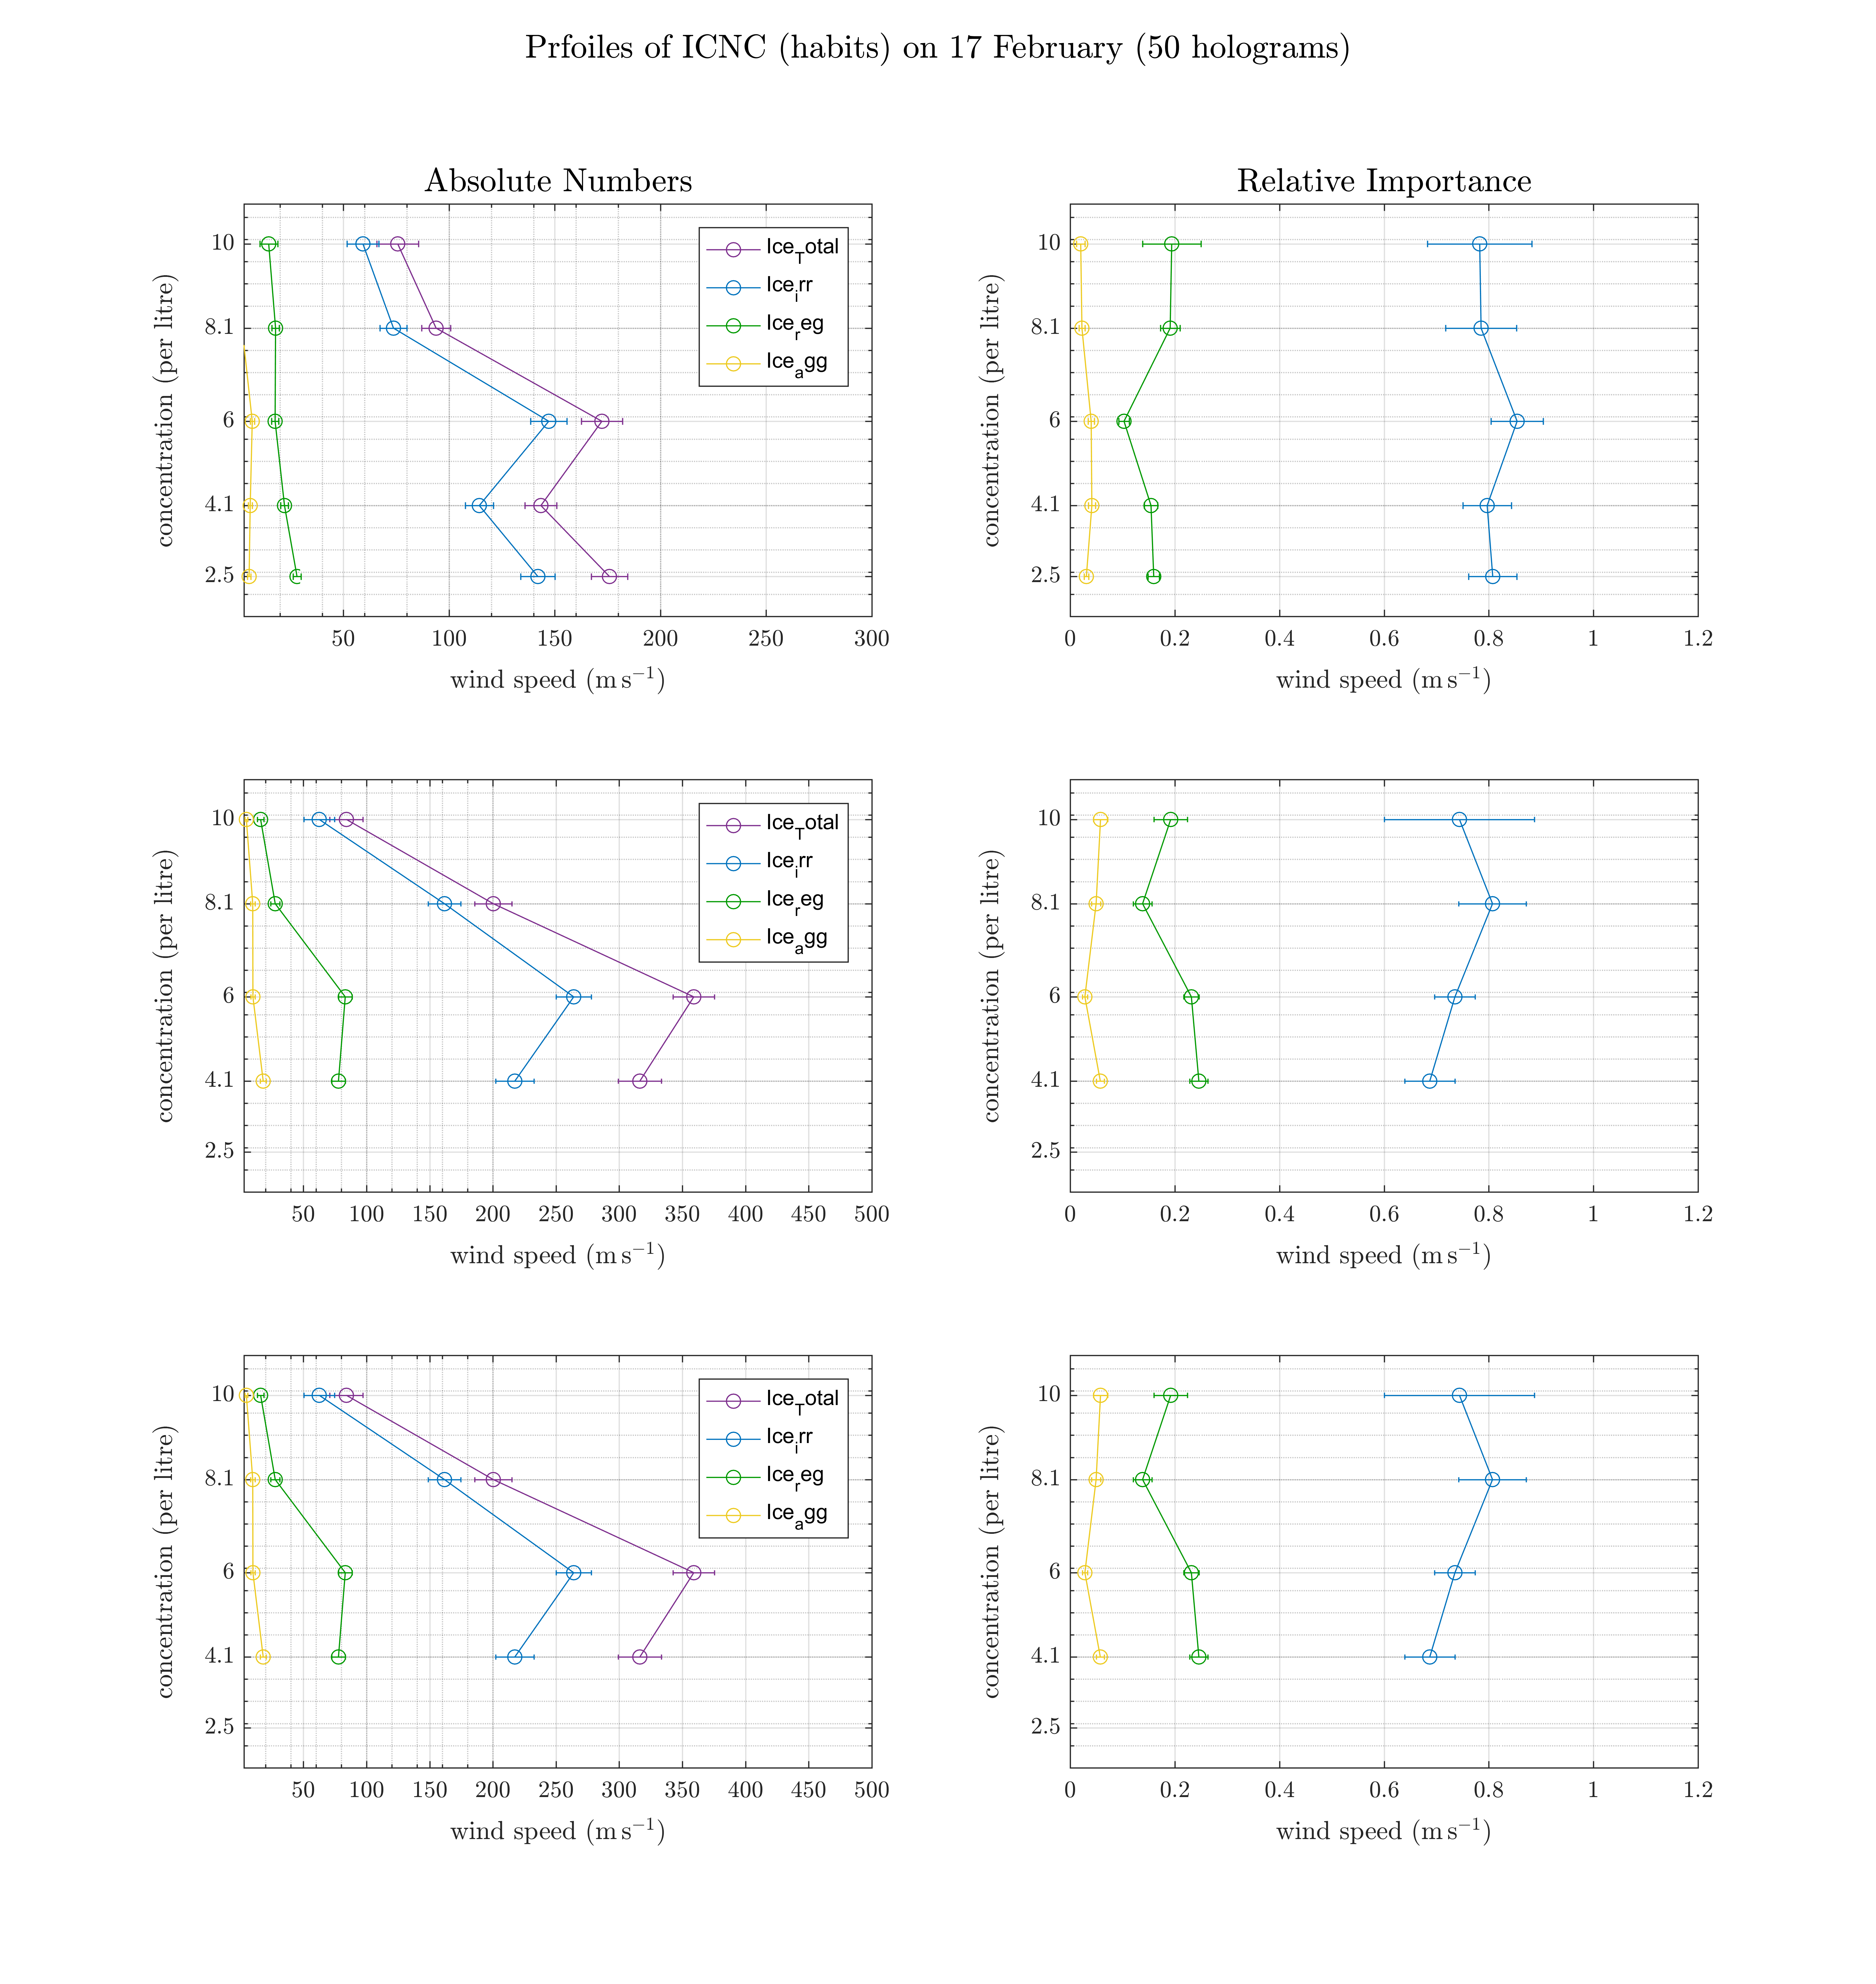
\includegraphics[width=14cm]{1702_habitsHeight.png}
 \caption{Vertical profiles of the concentration (left) and the relative importance (right) of the subclassified ice crystal habits: regular, irregular and aggregates. For the relative importance the number of ice crystals of different habits were divided by the total number of ice crystals. For theses plots the data as averaged over 50 holograms. In both cases the circles represent the mean of the 50 hologram averages. The error bars represent the standard error of the mean. }
 \label{fig:profilesHabits1702}
\end{figure}

\begin{figure}[h]
 \centering
 	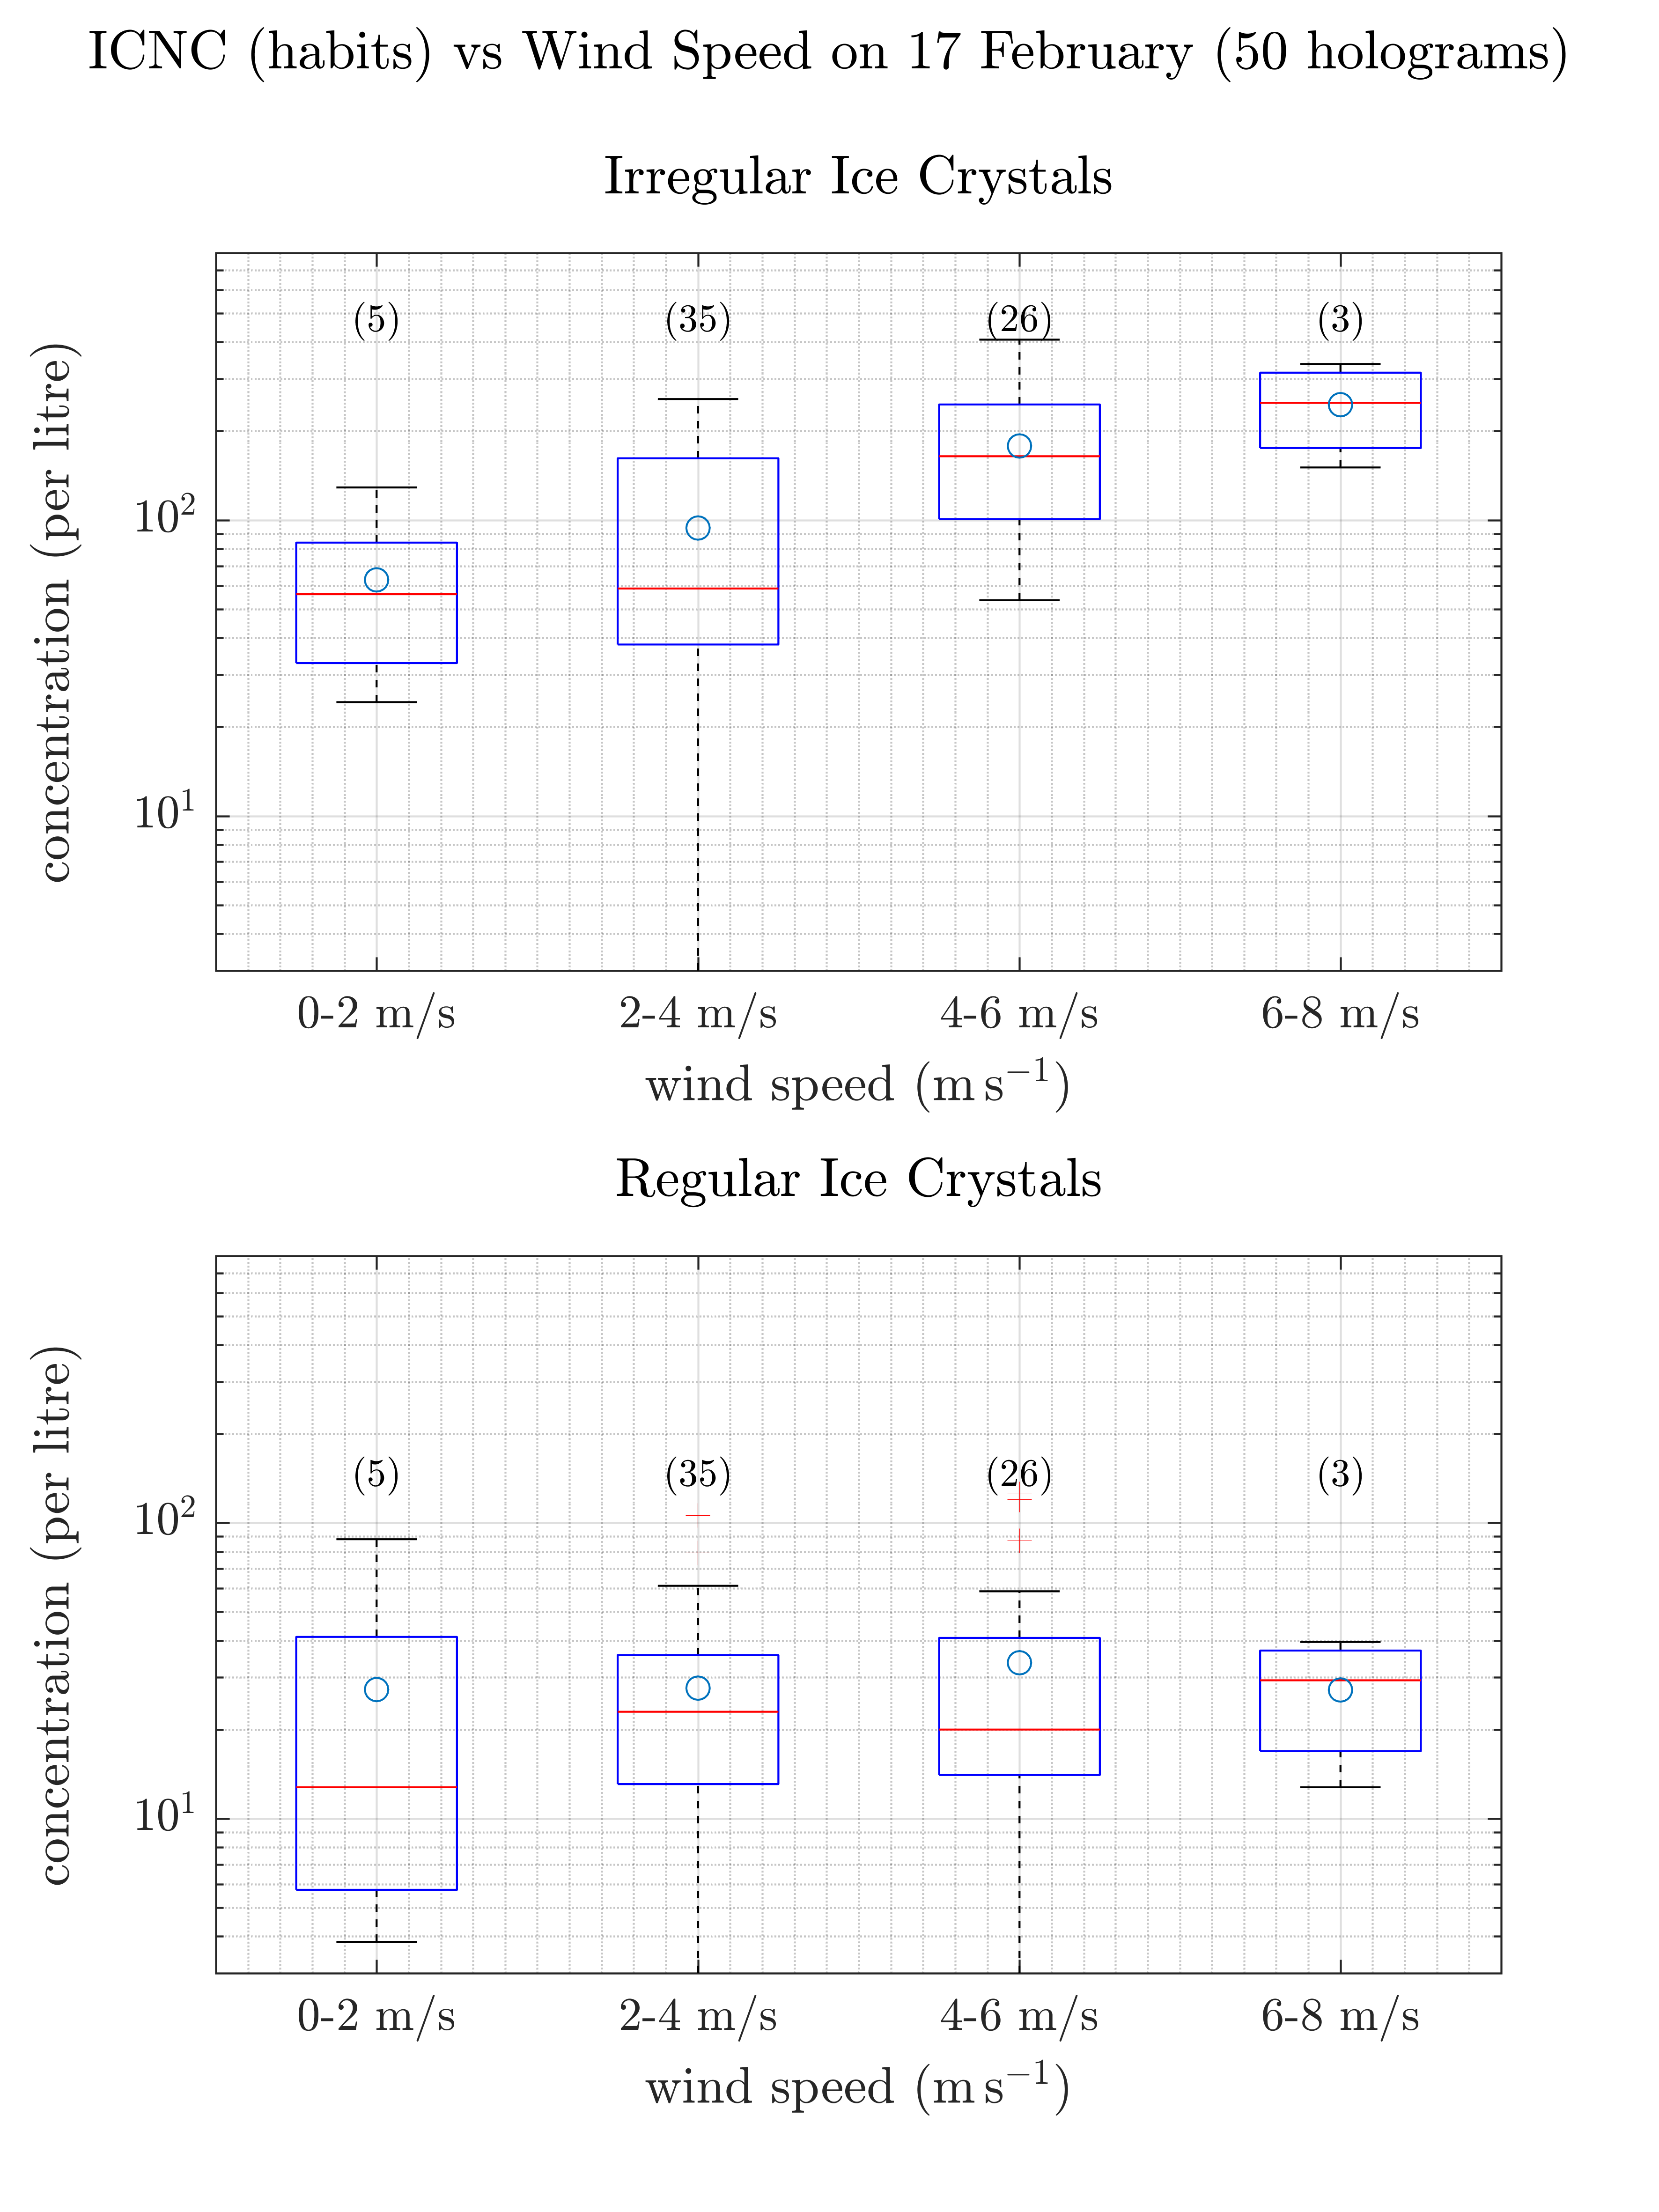
\includegraphics[width=14cm]{1702_habitswWS.png}
 \caption{As Figure \ref{fig:ICNCvsWSMAX0402} only for 17 February and different ice crystal habits as a function of the vertical wind speed.}
 \label{fig:ICNCvsWindHabits1702}
\end{figure}



%Text here ===>>>

%%

%  Numbered lines in equations:
%  To add line numbers to lines in equations,
%  \begin{linenomath*}
%  \begin{equation}
%  \end{equation}
%  \end{linenomath*}



%% Enter Figures and Tables near as possible to where they are first mentioned:
%
% DO NOT USE \psfrag or \subfigure commands.
%
% Figure captions go below the figure.
% Table titles go above tables;  other caption information
%  should be placed in last line of the table, using
% \multicolumn2l{$^a$ This is a table note.}
%
%----------------
% EXAMPLE FIGURE
%
% \begin{figure}[h]
% \centering
% when using pdflatex, use pdf file:
% 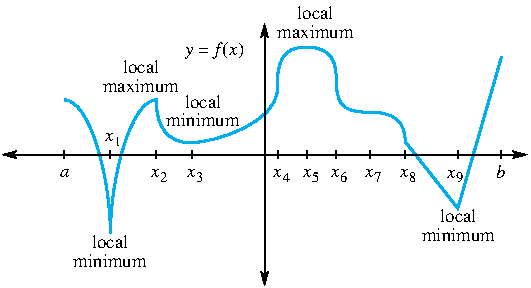
\includegraphics[width=20pc]{figsamp.pdf}
%
% when using dvips, use .eps file:
% 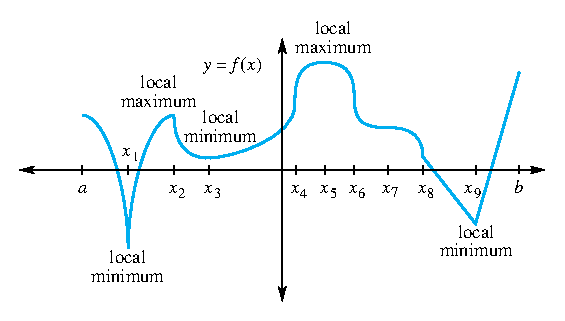
\includegraphics[width=20pc]{figsamp.eps}
%
% \caption{Short caption}
% \label{figone}
%  \end{figure}
%
% ---------------
% EXAMPLE TABLE
%
% \begin{table}
% \caption{Time of the Transition Between Phase 1 and Phase 2$^{a}$}
% \centering
% \begin{tabular}{l c}
% \hline
%  Run  & Time (min)  \\
% \hline
%   $l1$  & 260   \\
%   $l2$  & 300   \\
%   $l3$  & 340   \\
%   $h1$  & 270   \\
%   $h2$  & 250   \\
%   $h3$  & 380   \\
%   $r1$  & 370   \\
%   $r2$  & 390   \\
% \hline
% \multicolumn{2}{l}{$^{a}$Footnote text here.}
% \end{tabular}
% \end{table}

%% SIDEWAYS FIGURE and TABLE 
% AGU prefers the use of {sidewaystable} over {landscapetable} as it causes fewer problems.
%
% \begin{sidewaysfigure}
% 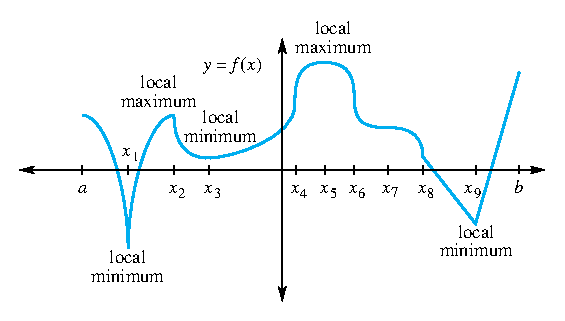
\includegraphics[width=20pc]{figsamp}
% \caption{caption here}
% \label{newfig}
% \end{sidewaysfigure}
% 
%  \begin{sidewaystable}
%  \caption{Caption here}
% \label{tab:signif_gap_clos}
%  \begin{tabular}{ccc}
% one&two&three\\
% four&five&six
%  \end{tabular}
%  \end{sidewaystable}

%% If using numbered lines, please surround equations with \begin{linenomath*}...\end{linenomath*}
%\begin{linenomath*}
%\begin{equation}
%y|{f} \sim g(m, \sigma),
%\end{equation}
%\end{linenomath*}

%%% End of body of article

%%%%%%%%%%%%%%%%%%%%%%%%%%%%%%%%
%% Optional Appendix goes here
%
% The \appendix command resets counters and redefines section heads
%
% After typing \appendix
%
%\section{Here Is Appendix Title}
% will show
% A: Here Is Appendix Title
%
%\appendix
%\section{Here is a sample appendix}

%%%%%%%%%%%%%%%%%%%%%%%%%%%%%%%%%%%%%%%%%%%%%%%%%%%%%%%%%%%%%%%%
%
% Optional Glossary, Notation or Acronym section goes here:
%
%%%%%%%%%%%%%%  
% Glossary is only allowed in Reviews of Geophysics
%  \begin{glossary}
%  \term{Term}
%   Term Definition here
%  \term{Term}
%   Term Definition here
%  \term{Term}
%   Term Definition here
%  \end{glossary}

%
%%%%%%%%%%%%%%
% Acronyms

 

%
%%%%%%%%%%%%%%
% Notation 
%   \begin{notation}
%   \notation{$a+b$} Notation Definition here
%   \notation{$e=mc^2$} 
%   Equation in German-born physicist Albert Einstein's theory of special
%  relativity that showed that the increased relativistic mass ($m$) of a
%  body comes from the energy of motion of the body—that is, its kinetic
%  energy ($E$)—divided by the speed of light squared ($c^2$).
%   \end{notation}




%%%%%%%%%%%%%%%%%%%%%%%%%%%%%%%%%%%%%%%%%%%%%%%%%%%%%%%%%%%%%%%%
%
%  ACKNOWLEDGMENTS
%
% The acknowledgments must list:
%
% •	All funding sources related to this work from all authors
%
% •	Any real or perceived financial conflicts of interests for any
%	author
%
% •	Other affiliations for any author that may be perceived as
% 	having a conflict of interest with respect to the results of this
% 	paper.
%
% •	A statement that indicates to the reader where the data
% 	supporting the conclusions can be obtained (for example, in the
% 	references, tables, supporting information, and other databases).
%
% It is also the appropriate place to thank colleagues and other contributors. 
% AGU does not normally allow dedications.




%% ------------------------------------------------------------------------ %%
%% Citations

% Please use ONLY \citet and \citep for reference citations.
% DO NOT use other cite commands (e.g., \cite, \citeyear, \nocite, \citealp, etc.).


%% Example \citet and \citep:
%  ...as shown by \citet{Boug10}, \citet{Buiz07}, \citet{Fra10},
%  \citet{Ghel00}, and \citet{Leit74}. 

%  ...as shown by \citep{Boug10}, \citep{Buiz07}, \citep{Fra10},
%  \citep{Ghel00, Leit74}. 

%  ...has been shown \citep [e.g.,][]{Boug10,Buiz07,Fra10}.



%%  REFERENCE LIST AND TEXT CITATIONS
%
% Either type in your references using
%
% \begin{thebibliography}{}
% \bibitem[{\textit{Kobayashi et~al.}}(2003)]{R2013} Kobayashi, T.,
% Tran, A.~H., Nishijo, H., Ono, T., and Matsumoto, G.  (2003).
% Contribution of hippocampal place cell activity to learning and
% formation of goal-directed navigation in rats. \textit{Neuroscience}
% 117, 1025--1035.
%
% \bibitem{}
% Text
% \end{thebibliography}
%
%%%%%%%%%%%%%%%%%%%%%%%%%%%%%%%%%%%%%%%%%%%%%%%
% Or, to use BibTeX:
%
% Follow these steps
%
% 1. Type in \bibliography{<name of your .bib file>} 
%    Run LaTeX on your LaTeX file.
%
% 2. Run BiBTeX on your LaTeX file.
%
% 3. Open the new .bbl file containing the reference list and
%   copy all the contents into your LaTeX file here.
%
% 4. Run LaTeX on your new file which will produce the citations.
%
% AGU does not want a .bib or a .bbl file. Please copy in the contents of your .bbl file here.


%% After you run BibTeX, Copy in the contents of the .bbl file here:

%%%%%%%%%%%%%%%%%%%%%%%%%%%%%%%%%%%%%%%%%%%%%%%%%%%%%%%%%%%%%%%%%%%%%
% Track Changes:
% To add words, \added{<word added>}
% To delete words, \deleted{<word deleted>}
% To replace words, \replace{<word to be replaced>}{<replacement word>}
% To explain why change was made: \explain{<explanation>} This will put
% a comment into the right margin.

%%%%%%%%%%%%%%%%%%%%%%%%%%%%%%%%%%%%%%%%%%%%%%%%%%%%%%%%%%%%%%%%%%%%%
% At the end of the document, use \listofchanges, which will list the
% changes and the page and line number where the change was made.

% When final version, \listofchanges will not produce anything,
% \added{<word or words>} word will be printed, \deleted{<word or words} will take away the word,
% \replaced{<delete this word>}{<replace with this word>} will print only the replacement word.
%  In the final version, \explain will not print anything.
%%%%%%%%%%%%%%%%%%%%%%%%%%%%%%%%%%%%%%%%%%%%%%%%%%%%%%%%%%%%%%%%%%%%%

%%%
\listofchanges
%%%

\end{document}

%%%%%%%%%%%%%%%%%%%%%%%%%%%%%%%%%%%%%
%% Supporting Information
%% (Optional) See AGUSuppInfoSamp.tex/pdf for requirements 
%% for Supporting Information.
%%%%%%%%%%%%%%%%%%%%%%%%%%%%%%%%%%%%%



%%%%%%%%%%%%%%%%%%%%%%%%%%%%%%%%%%%%%%%%%%%%%%%%%%%%%%%%%%%%%%%

More Information and Advice:

%% ------------------------------------------------------------------------ %%
%
%  SECTION HEADS
%
%% ------------------------------------------------------------------------ %%

% Capitalize the first letter of each word (except for
% prepositions, conjunctions, and articles that are
% three or fewer letters).

% AGU follows standard outline style; therefore, there cannot be a section 1 without
% a section 2, or a section 2.3.1 without a section 2.3.2.
% Please make sure your section numbers are balanced.
% ---------------
% Level 1 head
%
% Use the \section{} command to identify level 1 heads;
% type the appropriate head wording between the curly
% brackets, as shown below.
%
%An example:
%\section{Level 1 Head: Introduction}
%
% ---------------
% Level 2 head
%
% Use the \subsection{} command to identify level 2 heads.
%An example:
%\subsection{Level 2 Head}
%
% ---------------
% Level 3 head
%
% Use the \subsubsection{} command to identify level 3 heads
%An example:
%\subsubsection{Level 3 Head}
%
%---------------
% Level 4 head
%
% Use the \subsubsubsection{} command to identify level 3 heads
% An example:
%\subsubsubsection{Level 4 Head} An example.
%
%% ------------------------------------------------------------------------ %%
%
%  IN-TEXT LISTS
%
%% ------------------------------------------------------------------------ %%
%
% Do not use bulleted lists; enumerated lists are okay.
% \begin{enumerate}
% \item
% \item
% \item
% \end{enumerate}
%
%% ------------------------------------------------------------------------ %%
%
%  EQUATIONS
%
%% ------------------------------------------------------------------------ %%

% Single-line equations are centered.
% Equation arrays will appear left-aligned.

Math coded inside display math mode \[ ...\]
 will not be numbered, e.g.,:
 \[ x^2=y^2 + z^2\]

 Math coded inside \begin{equation} and \end{equation} will
 be automatically numbered, e.g.,:
 \begin{equation}
 x^2=y^2 + z^2
 \end{equation}


% To create multiline equations, use the
% \begin{eqnarray} and \end{eqnarray} environment
% as demonstrated below.
\begin{eqnarray}
  x_{1} & = & (x - x_{0}) \cos \Theta \nonumber \\
        && + (y - y_{0}) \sin \Theta  \nonumber \\
  y_{1} & = & -(x - x_{0}) \sin \Theta \nonumber \\
        && + (y - y_{0}) \cos \Theta.
\end{eqnarray}

%If you don't want an equation number, use the star form:
%\begin{eqnarray*}...\end{eqnarray*}

% Break each line at a sign of operation
% (+, -, etc.) if possible, with the sign of operation
% on the new line.

% Indent second and subsequent lines to align with
% the first character following the equal sign on the
% first line.

% Use an \hspace{} command to insert horizontal space
% into your equation if necessary. Place an appropriate
% unit of measure between the curly braces, e.g.
% \hspace{1in}; you may have to experiment to achieve
% the correct amount of space.


%% ------------------------------------------------------------------------ %%
%
%  EQUATION NUMBERING: COUNTER
%
%% ------------------------------------------------------------------------ %%

% You may change equation numbering by resetting
% the equation counter or by explicitly numbering
% an equation.

% To explicitly number an equation, type \eqnum{}
% (with the desired number between the brackets)
% after the \begin{equation} or \begin{eqnarray}
% command.  The \eqnum{} command will affect only
% the equation it appears with; LaTeX will number
% any equations appearing later in the manuscript
% according to the equation counter.
%

% If you have a multiline equation that needs only
% one equation number, use a \nonumber command in
% front of the double backslashes (\\) as shown in
% the multiline equation above.

% If you are using line numbers, remember to surround
% equations with \begin{linenomath*}...\end{linenomath*}

%  To add line numbers to lines in equations:
%  \begin{linenomath*}
%  \begin{equation}
%  \end{equation}
%  \end{linenomath*}



